\documentclass[11pt]{article}
\usepackage[margin=1in]{geometry}
\usepackage[T1]{fontenc}
\usepackage[utf8]{inputenc}
\usepackage{lmodern}
\usepackage{booktabs}
\usepackage{enumitem}
\usepackage{hyperref}
\usepackage{graphicx}
\usepackage[
  backend=biber,
  style=numeric,
  sorting=none,
  giveninits=true,
  maxbibnames=3,
  minbibnames=1,
  maxcitenames=2,
  doi=false,
  url=false,
  isbn=false,
  eprint=false
]{biblatex}

\addbibresource{zzzaurak.bib}

\hypersetup{hidelinks}

\newcommand{\code}[1]{\texttt{#1}}

\title{ObsAstro26 P2Rp4: Supernova Data Analysis Report}
\author{Group 1}
\date{June 3, 2026}

\begin{document}
\maketitle

\section*{Contributions}
\addcontentsline{toc}{section}{Contributions}
\medskip
\noindent\begin{tabular}{p{0.28\linewidth}p{0.20\linewidth}p{0.44\linewidth}}
\toprule
Task & Person & Contribution \\
\midrule
introduction,scientific background & Linlin & \dots \\

target selection \& observation preparations & Minxuan He & \dots \\

data reduction and analyses & Ziheng Zhang & Organized reduced 1D BFOSC spectra from Ruifeng Huang; compiled TNS redshifts; measured sparse-spectrum lines; produced QC tables, figures, and qualitative TARDIS comparisons. \\

results and conclusion (\& summary) & Xinyu Liu & \dots \\

\bottomrule
\end{tabular}

\tableofcontents
\newpage

\section{Scientific Question}

\section{Data}

\section{Data Reduction and Analyses}
The analysis starts from one-dimensional BFOSC FITS spectra in the project, including 5 targets and 12 spectra. For each supernova, the final spectrum was obtained by our group with the Xinglong 2.16 m telescope on 2026 May 8. The other epochs were reduced spectra delivered by Ruifeng Huang. This work therefore did not redo the two-dimensional reduction steps, such as bias and flat-field correction, cosmic-ray rejection, two-dimensional wavelength calibration, sky subtraction, and one-dimensional extraction. Those basic reduction steps had already been completed before the spectra were delivered.

BFOSC is a low-resolution imaging and spectroscopic instrument on the Xinglong 2.16 m telescope, with a typical low-resolution spectral resolving power of about $R\sim500$--$2000$ \cite{fanXinglong216m2016,zhaoBFOSCEfficiency2018}. A closely related reference for this project is the spectral data release by the Tsinghua Supernova Group led by Xiaofeng Wang, which includes many Type II supernova spectra obtained with the Xinglong 2.16 m telescope and the Lijiang 2.4 m telescope, and measures line identifications, velocities, and pEW values in a systematic way \cite{linSpectralDataRelease2024}. Following such work, standard long-slit supernova spectral reduction usually includes CCD bias and bad-pixel treatment, flat-field correction, arc-lamp wavelength calibration, sky subtraction, one-dimensional extraction, relative flux calibration from a standard star or instrumental response, and atmospheric absorption or relative-response correction when needed. The spectra used here are products after these steps, so the subsequent analysis does not include a full original-reduction error budget.

Target classifications, discovery dates, and redshifts are primarily taken from the public TNS data. This project does not manually remeasure the redshift. The public TNS data do not provide maximum-light or peak-date fields, so all phases in this section are days since TNS discovery, not phases relative to maximum light. For targets with a TNS redshift, the observed wavelength is transformed to the rest frame using
\[
\lambda_{\rm rest}=\frac{\lambda_{\rm obs}}{1+z_{\rm TNS}}.
\]
SN2026LMP does not have a reliable TNS redshift, so it is retained only for qualitative line-shape checks and is not used for any quantitative velocity or pEW conclusion.

The project code is available in the \href{https://github.com/Zzzaurak/obsastro-sn-pipeline}{GitHub repository}. The main analysis in this section is implemented in \path{src/spectral_pipeline.py} and \path{src/spectral_notebook_tools.py}, with \path{notebooks/02_spectral_analysis_pipeline.ipynb} as the interactive inspection interface. The classification and template-comparison logic follows the general practice of SNID and WISeREP-based public spectral comparison work \cite{blondinDeterminingTypeRedshift2007,yaronWISeREPInteractiveSupernova2012}.

\subsection{Classifications, Redshifts, and Adopted Line List}
To avoid including weak lines, blended lines, and targets without redshift in quantitative conclusions, the adopted line list is conservative after manual inspection. For the Type Ia targets SN2026FVX and SN2026JLM, Ca II H\&K and Si II 6355 are adopted. Si II 5972 is sensitive to the local window and can have its pEW contaminated by the broad Si II 6355 absorption, so it is not included in the final adopted list. For the Type II target SN2026KID, only Fe II 5169 is adopted as an expansion-velocity indicator. H$\alpha$ and H$\beta$ are affected by P-Cygni emission, noise, and local-continuum placement in these spectra, so they are not automatically adopted as velocity measurements. For the single-epoch SN Ic target SN2026KIE, Ca II H\&K, Ca II NIR, and O I 7774 are adopted, although the Ca II NIR feature is shallow and is interpreted only as supporting evidence. SN2026LMP is roughly consistent with a SN IIb classification, but it lacks a TNS redshift; all candidate lines are therefore kept as \code{check}.

\begin{table}[htbp]
\centering
\caption{Target-level status and adopted line list used in this section. Phases are days since TNS discovery. From code by Ziheng Zhang.}
\label{tab:target-status}
\resizebox{\linewidth}{!}{%
\begin{tabular}{llcccl}
\toprule
Target & Type & Redshift & Spectra & Phase range (d) & Adopted lines \\
\midrule
SN2026FVX & SN Ia & 0.004846 & 4 & 1.7--51.6 & CaIIHK, SiII6355 \\
SN2026JLM & SN Ia & 0.016738 & 3 & 14.5--26.6 & CaIIHK, SiII6355 \\
SN2026KID & SN II & 0.0017 & 3 & 4.0--16.1 & FeII5169 \\
SN2026KIE & SN Ic & 0.00424 & 1 & 16.3--16.3 & CaIIHK, CaIINIR, OI7774 \\
SN2026LMP & SN IIb & -- & 1 & -- & none \\
\bottomrule
\end{tabular}}
\end{table}

\begin{figure}[htbp]
\centering
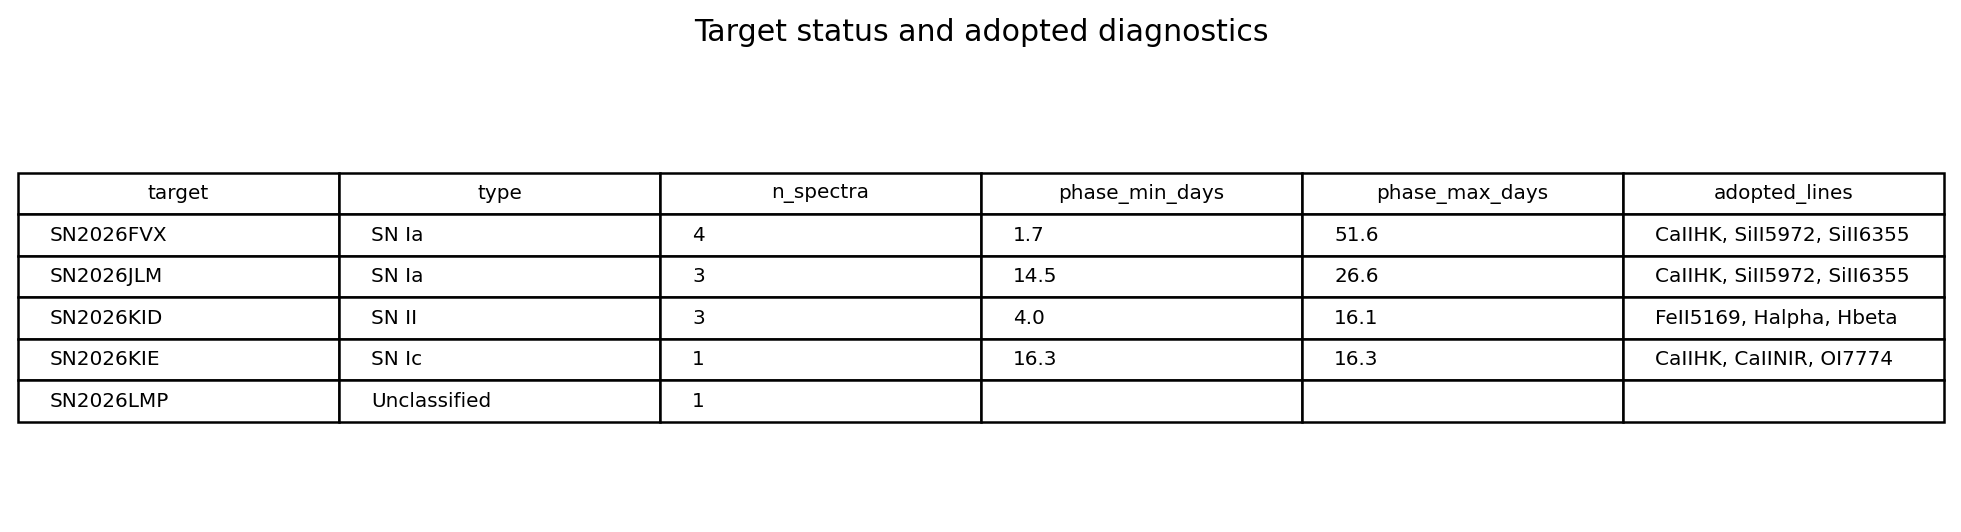
\includegraphics[width=0.96\linewidth]{images_zzzaurak/target_status_table.png}
\caption{Target-level status table. Because SN2026LMP lacks a reliable TNS redshift, it is retained only for qualitative inspection and is not used for quantitative velocity or pEW conclusions. From code by Ziheng Zhang.}
\label{fig:target-status}
\end{figure}

\subsection{Line-Measurement Algorithm}
For each candidate absorption line, a local window is cut in the rest frame. A Savitzky--Golay filter is used to suppress pixel-scale noise, and median points near the two window edges define a local linear continuum. The normalized spectrum is
\[
f_{\rm norm}(\lambda)=\frac{f_{\rm smooth}(\lambda)}{f_{\rm cont}(\lambda)}.
\]
Following Yi Yang's suggestion, the absorption center is not measured with a Gaussian profile fit. Instead, the adopted absorption wavelength is the local trough minimum in the normalized spectrum:
\[
\lambda_{\rm min}=\arg\min f_{\rm norm}(\lambda).
\]
The velocity and line depth are then defined as
\[
v=c\frac{\lambda_0-\lambda_{\rm min}}{\lambda_0}, \qquad
d=1-f_{\rm norm}(\lambda_{\rm min}),
\]
where $\lambda_0$ is the laboratory rest wavelength. The FWHM is measured non-parametrically. At the half-depth level
\[
f_{1/2}=1-\frac{d}{2},
\]
the code searches for the left and right linear-interpolation crossings, $\lambda_{\rm L}$ and $\lambda_{\rm R}$, and defines
\[
{\rm FWHM}=\lambda_{\rm R}-\lambda_{\rm L}.
\]
The pEW is the direct positive absorption area below the normalized continuum:
\[
{\rm pEW}=\int_{\lambda_1}^{\lambda_2}\max\left[1-f_{\rm norm}(\lambda),0\right]\,d\lambda.
\]
This trough-minimum method is more direct than a Gaussian-center fit and is closer to the way broad absorption troughs are checked by eye. The Si II and Ca II velocities and pEW values of the Type Ia targets are mainly compared with BSNIP and CSP-style samples \cite{silvermanBerkeleySupernovaIa2012a,folatelliSPECTROSCOPYTYPEIa2013,zhaoInvestigationFWHMAbsorption2026}. The Type II and stripped-envelope targets are compared with Type II and stripped-envelope spectral samples \cite{gutierrezTypeIISupernova2017,linSpectralDataRelease2024,modjazOPTICALSPECTRA732014,xiangSpectralDatasetStrippedenvelope2026}.

The plotted error bars are formal statistical uncertainties. The velocity uncertainty is propagated from the uncertainty of the trough wavelength, which is estimated from the local residual noise and wavelength sampling. The pEW uncertainty is propagated from the local normalized residual noise over the integration region. The FWHM uncertainty is estimated at the sampling level near the half-depth crossings.

The pipeline also records \code{velocity\_sys\_kms}, \code{pEW\_sys\_A}, and \code{FWHM\_sys\_A}, which describe the empirical scatter under changes to the smoothing window and continuum-edge fraction. These estimates are still not a complete error budget, because they do not fully include TNS redshift uncertainty, wavelength-calibration systematics, line blending, or atmospheric and instrument response effects.

\subsection{Manual Inspection and Adopted-Measurement Rules}
After the automatic measurements, the local diagnostic plots were inspected target by target. In these plots, the gray curve is the local raw spectrum, the black curve is the smoothed spectrum, the orange curve is the local continuum, the red dashed line is the laboratory rest wavelength, the green dashed line is the adopted trough minimum, and the purple shading marks only the pEW integration region, not a Gaussian model.

The manual inspection applied three main decisions. First, lines that are easily blended were removed or downgraded; for example, the pEW of Si II 5972 can be contaminated by Si II 6355, so it is removed from the final adopted list. Second, unstable automatic Balmer velocities were removed. For SN2026KID, the H$\alpha$ and H$\beta$ trough minima are affected by emission structure, noise, and local-continuum placement, so they are not adopted. Third, targets without a redshift are not used quantitatively: even if candidate features are visible in SN2026LMP, they are all marked as \code{check}.

The final \path{line_diagnostics_qc.csv} table contains 28 candidate measurements, including 18 \code{adopt} rows and 10 \code{check} rows. Narrow or clearly unreliable automatic troughs are kept as \code{check}, including Ca II H\&K for SN2026FVX on 2026 March 26, Ca II H\&K for SN2026JLM on 2026 May 4, and all candidate features in SN2026LMP.

More specifically, the three adopted Fe II 5169 points for SN2026KID are shallow, the Ca II NIR pEW uncertainty for SN2026KIE is larger than the measurement itself, and the early Ca II H\&K pEW values for SN2026FVX and SN2026JLM are sensitive to continuum placement. These points can still support the velocity scale or line identification, but they should not be over-interpreted in pEW or FWHM. A stricter final table could add a pEW signal-to-noise or systematics threshold and downgrade these weak \code{adopt} rows to \code{check}, at the cost of reducing early Ia Ca II and core-collapse velocity coverage.

\begin{figure}[htbp]
\centering
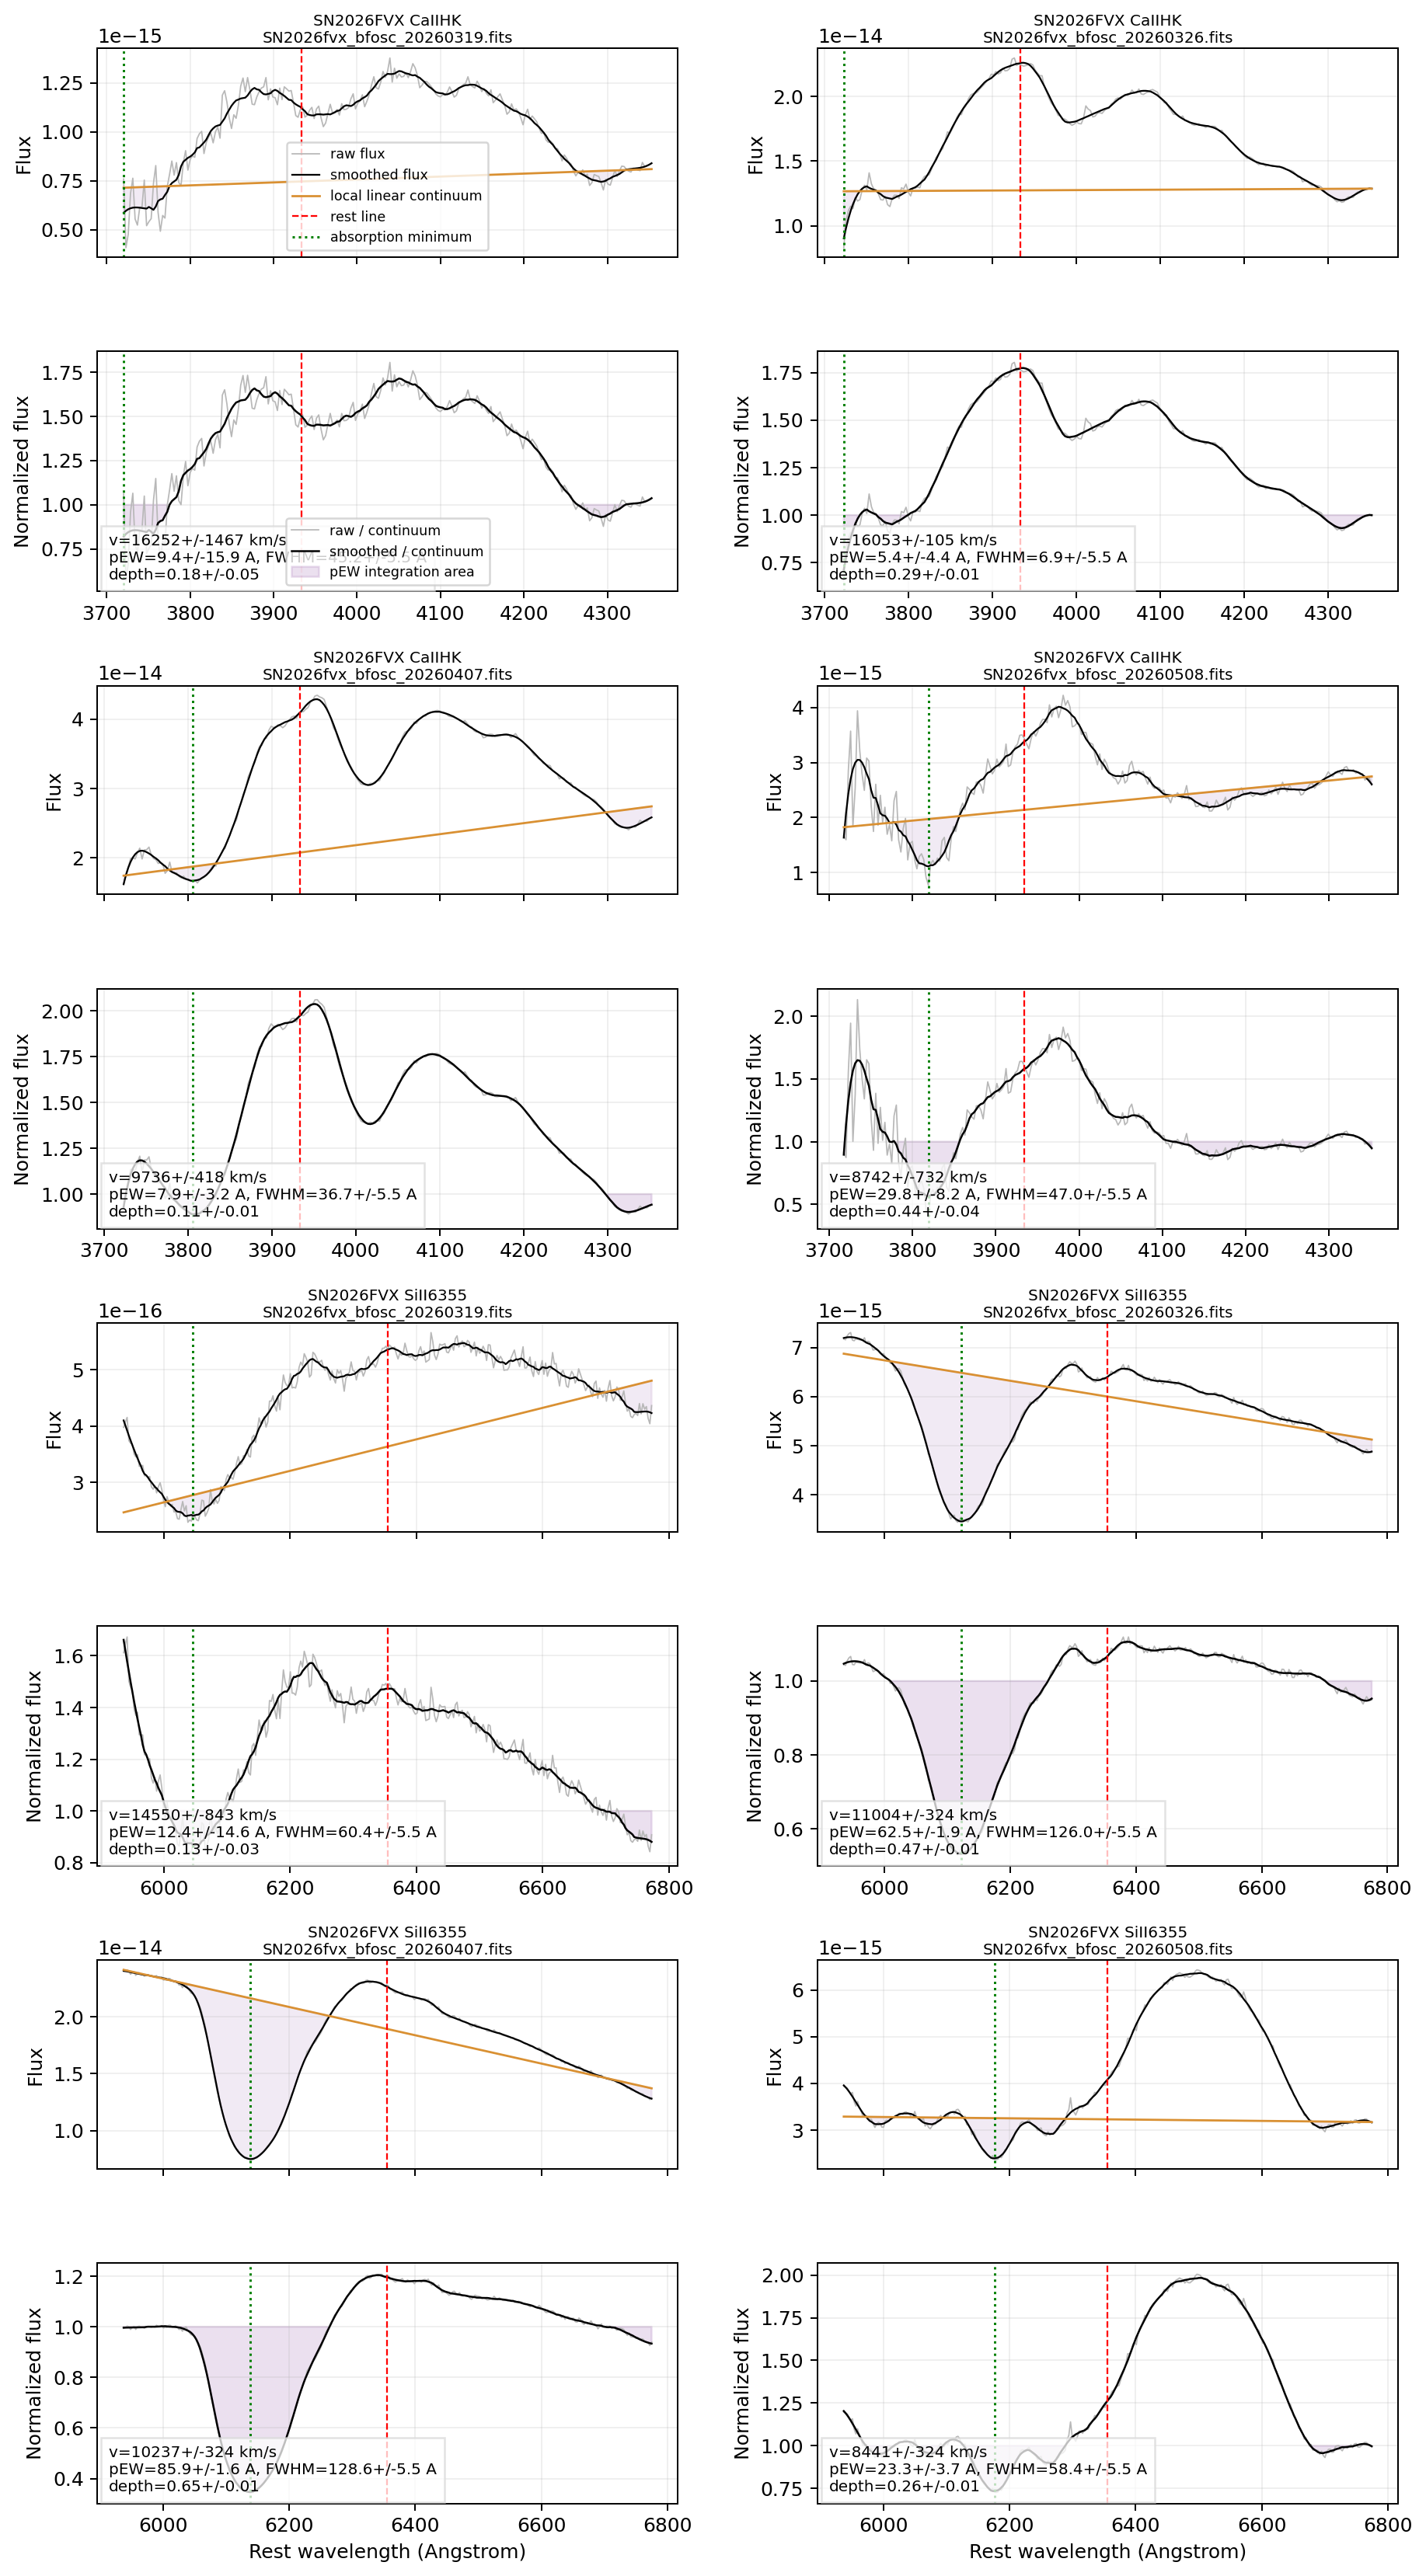
\includegraphics[width=0.96\linewidth,height=0.68\textheight,keepaspectratio]{images_zzzaurak/SN2026FVX_line_diagnostics_grid.png}
\caption{Local line-diagnostic plot for SN2026FVX. The green dashed line marks the trough-minimum absorption center, and the purple region marks the pEW integration region. From code by Ziheng Zhang.}
\label{fig:fvx-line-grid}
\end{figure}

\begin{figure}[htbp]
\centering
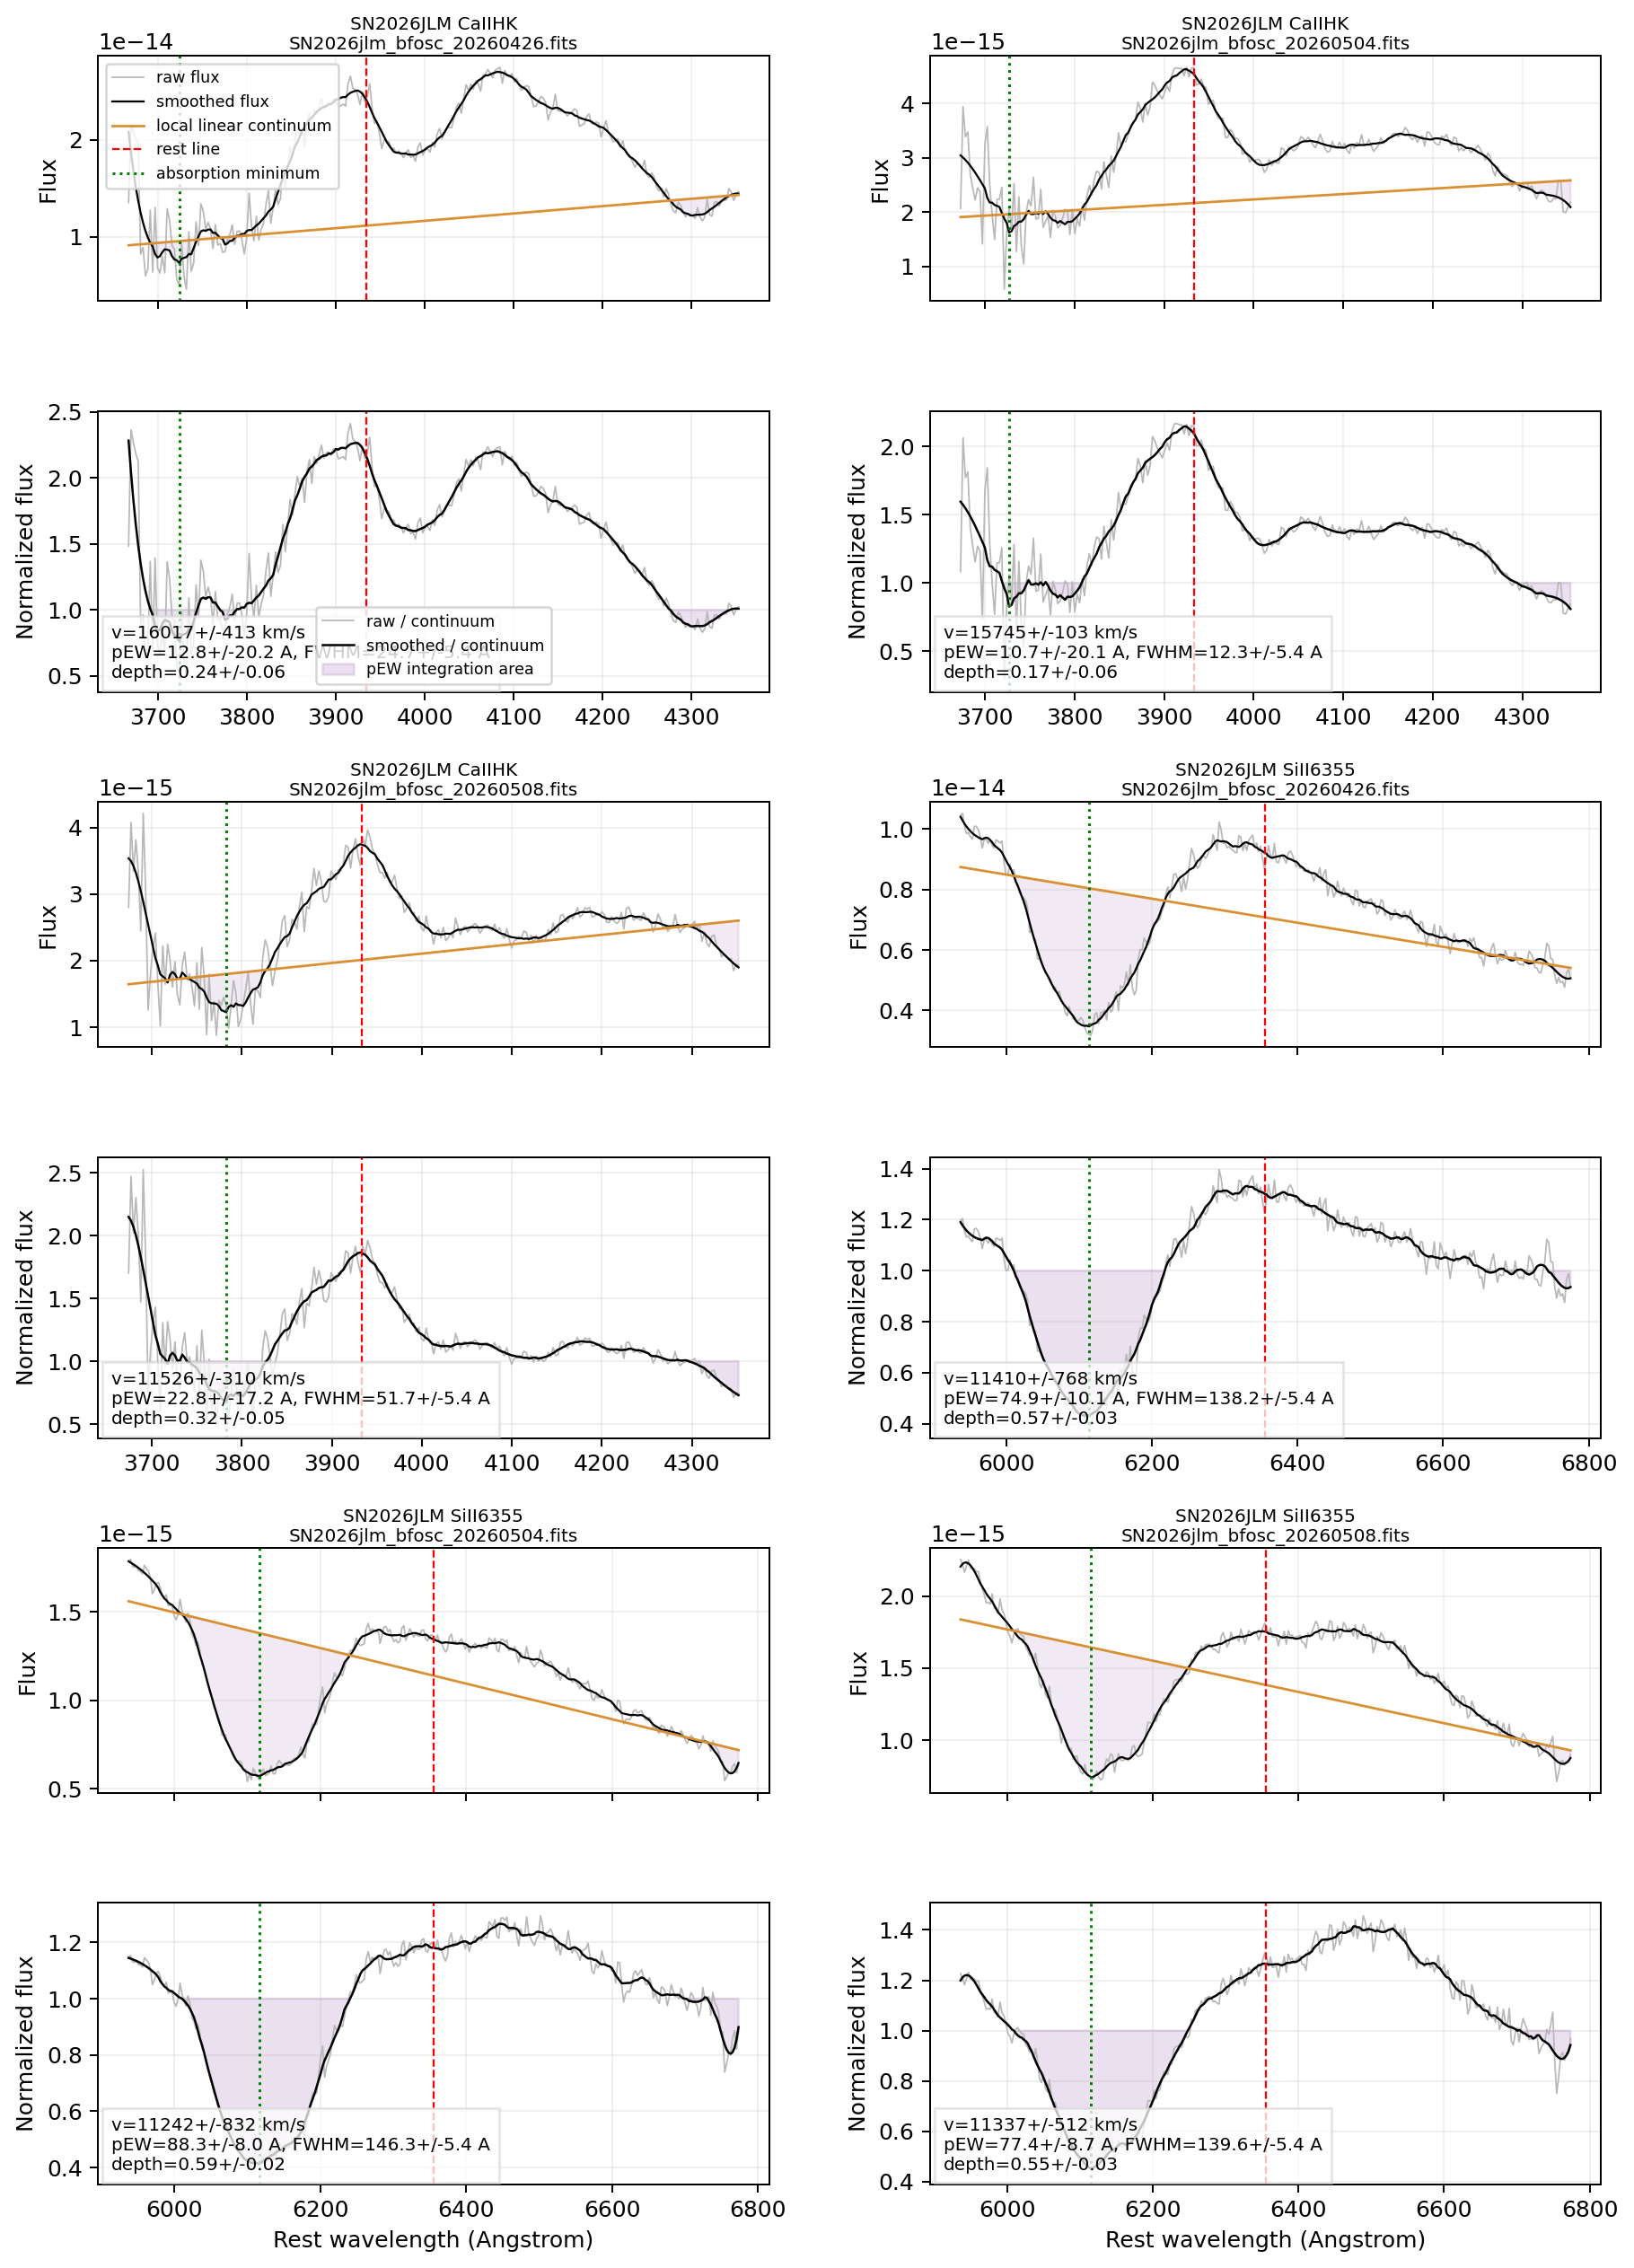
\includegraphics[width=0.96\linewidth,height=0.68\textheight,keepaspectratio]{images_zzzaurak/SN2026JLM_line_diagnostics_grid.png}
\caption{Local line-diagnostic plot for SN2026JLM. Si II 6355 is the most stable Type Ia velocity indicator for this target. From code by Ziheng Zhang.}
\label{fig:jlm-line-grid}
\end{figure}

\begin{figure}[htbp]
\centering
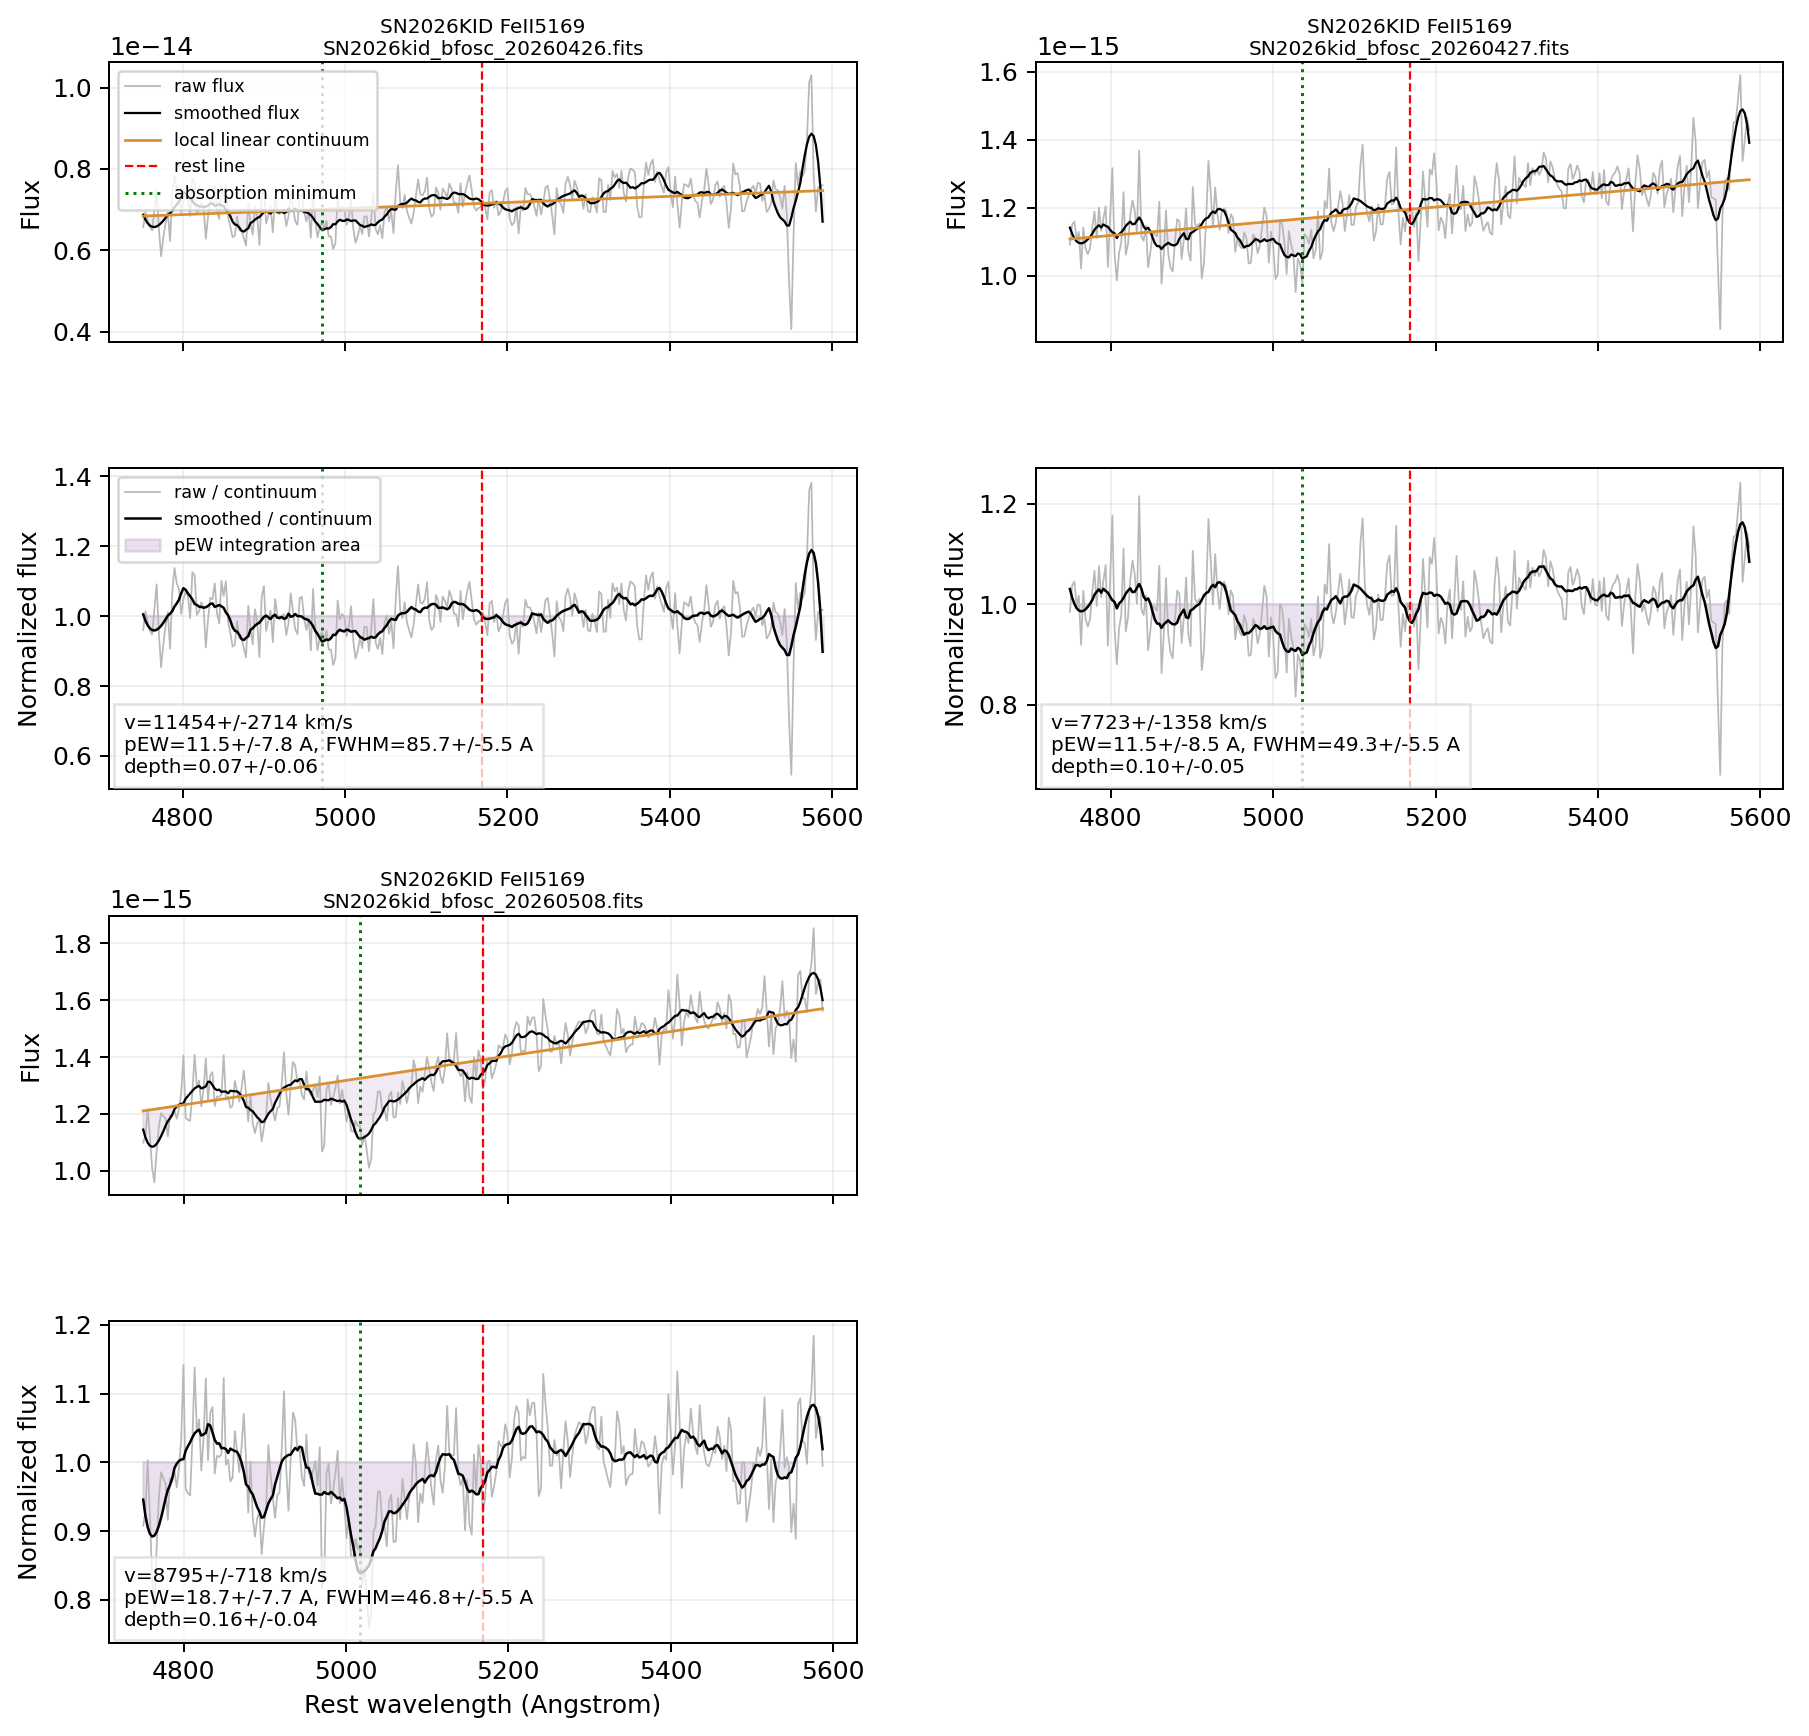
\includegraphics[width=0.96\linewidth,height=0.68\textheight,keepaspectratio]{images_zzzaurak/SN2026KID_line_diagnostics_grid.png}
\caption{Local line-diagnostic plot for SN2026KID. Fe II 5169 is used as the Type II velocity-scale indicator, while Balmer lines are kept only for morphology checks. From code by Ziheng Zhang.}
\label{fig:kid-line-grid}
\end{figure}

\begin{figure}[htbp]
\centering
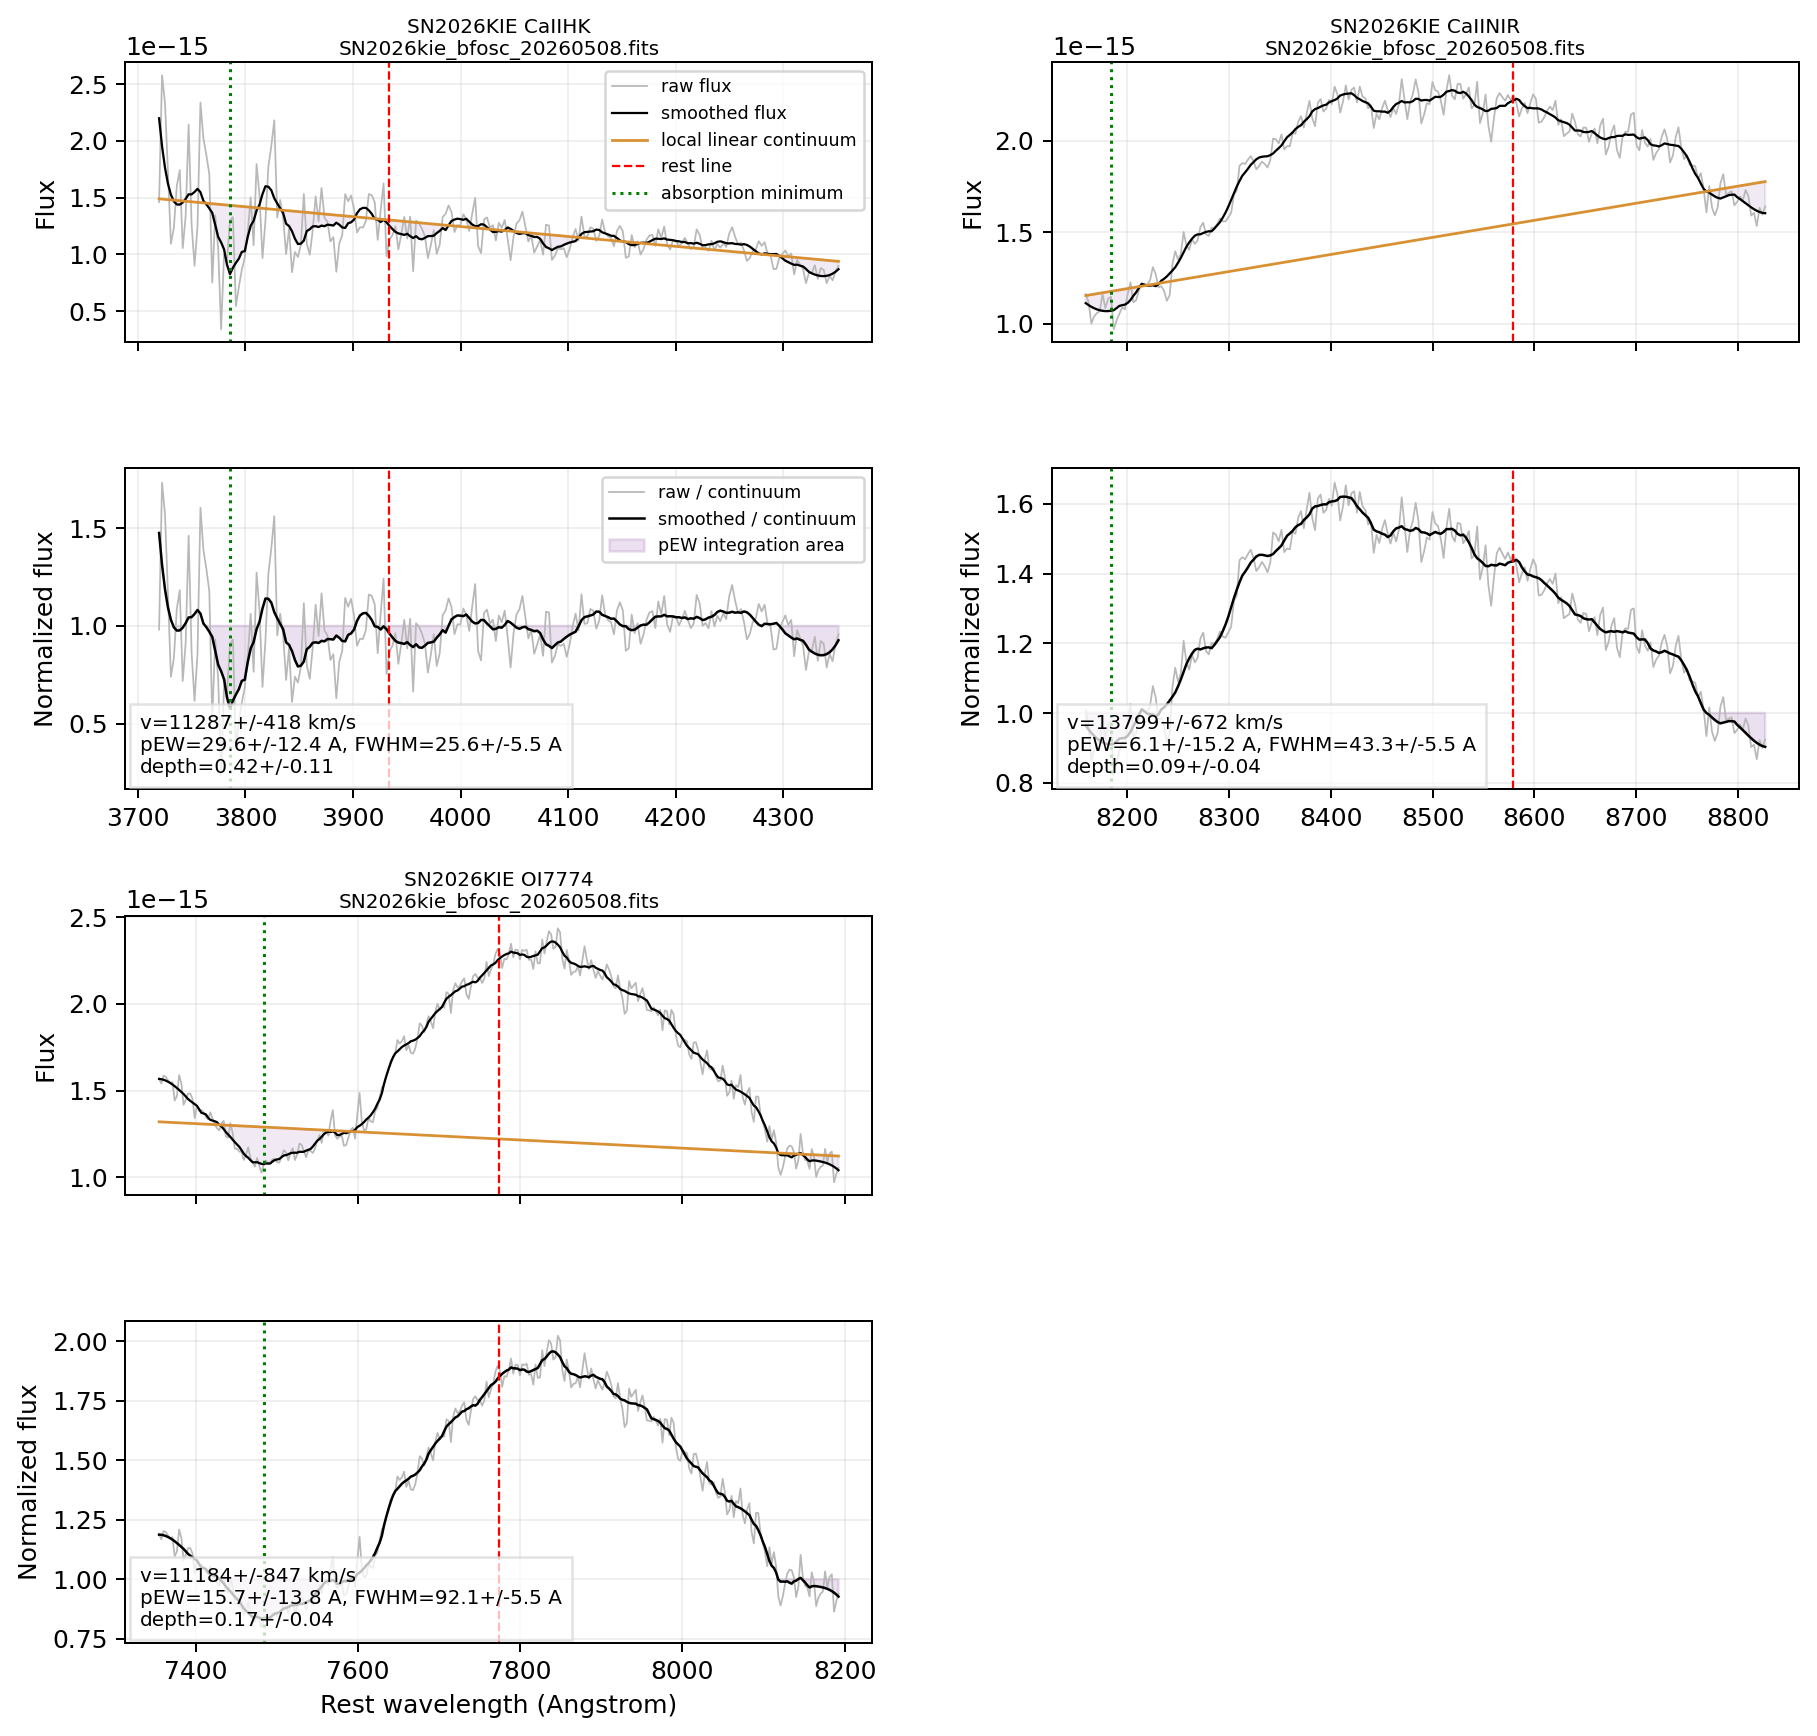
\includegraphics[width=0.96\linewidth,height=0.68\textheight,keepaspectratio]{images_zzzaurak/SN2026KIE_line_diagnostics_grid.png}
\caption{Single-epoch local line-diagnostic plot for SN2026KIE. Ca II and O I support the stripped-envelope classification but cannot constrain time evolution. From code by Ziheng Zhang.}
\label{fig:kie-line-grid}
\end{figure}

\begin{figure}[htbp]
\centering
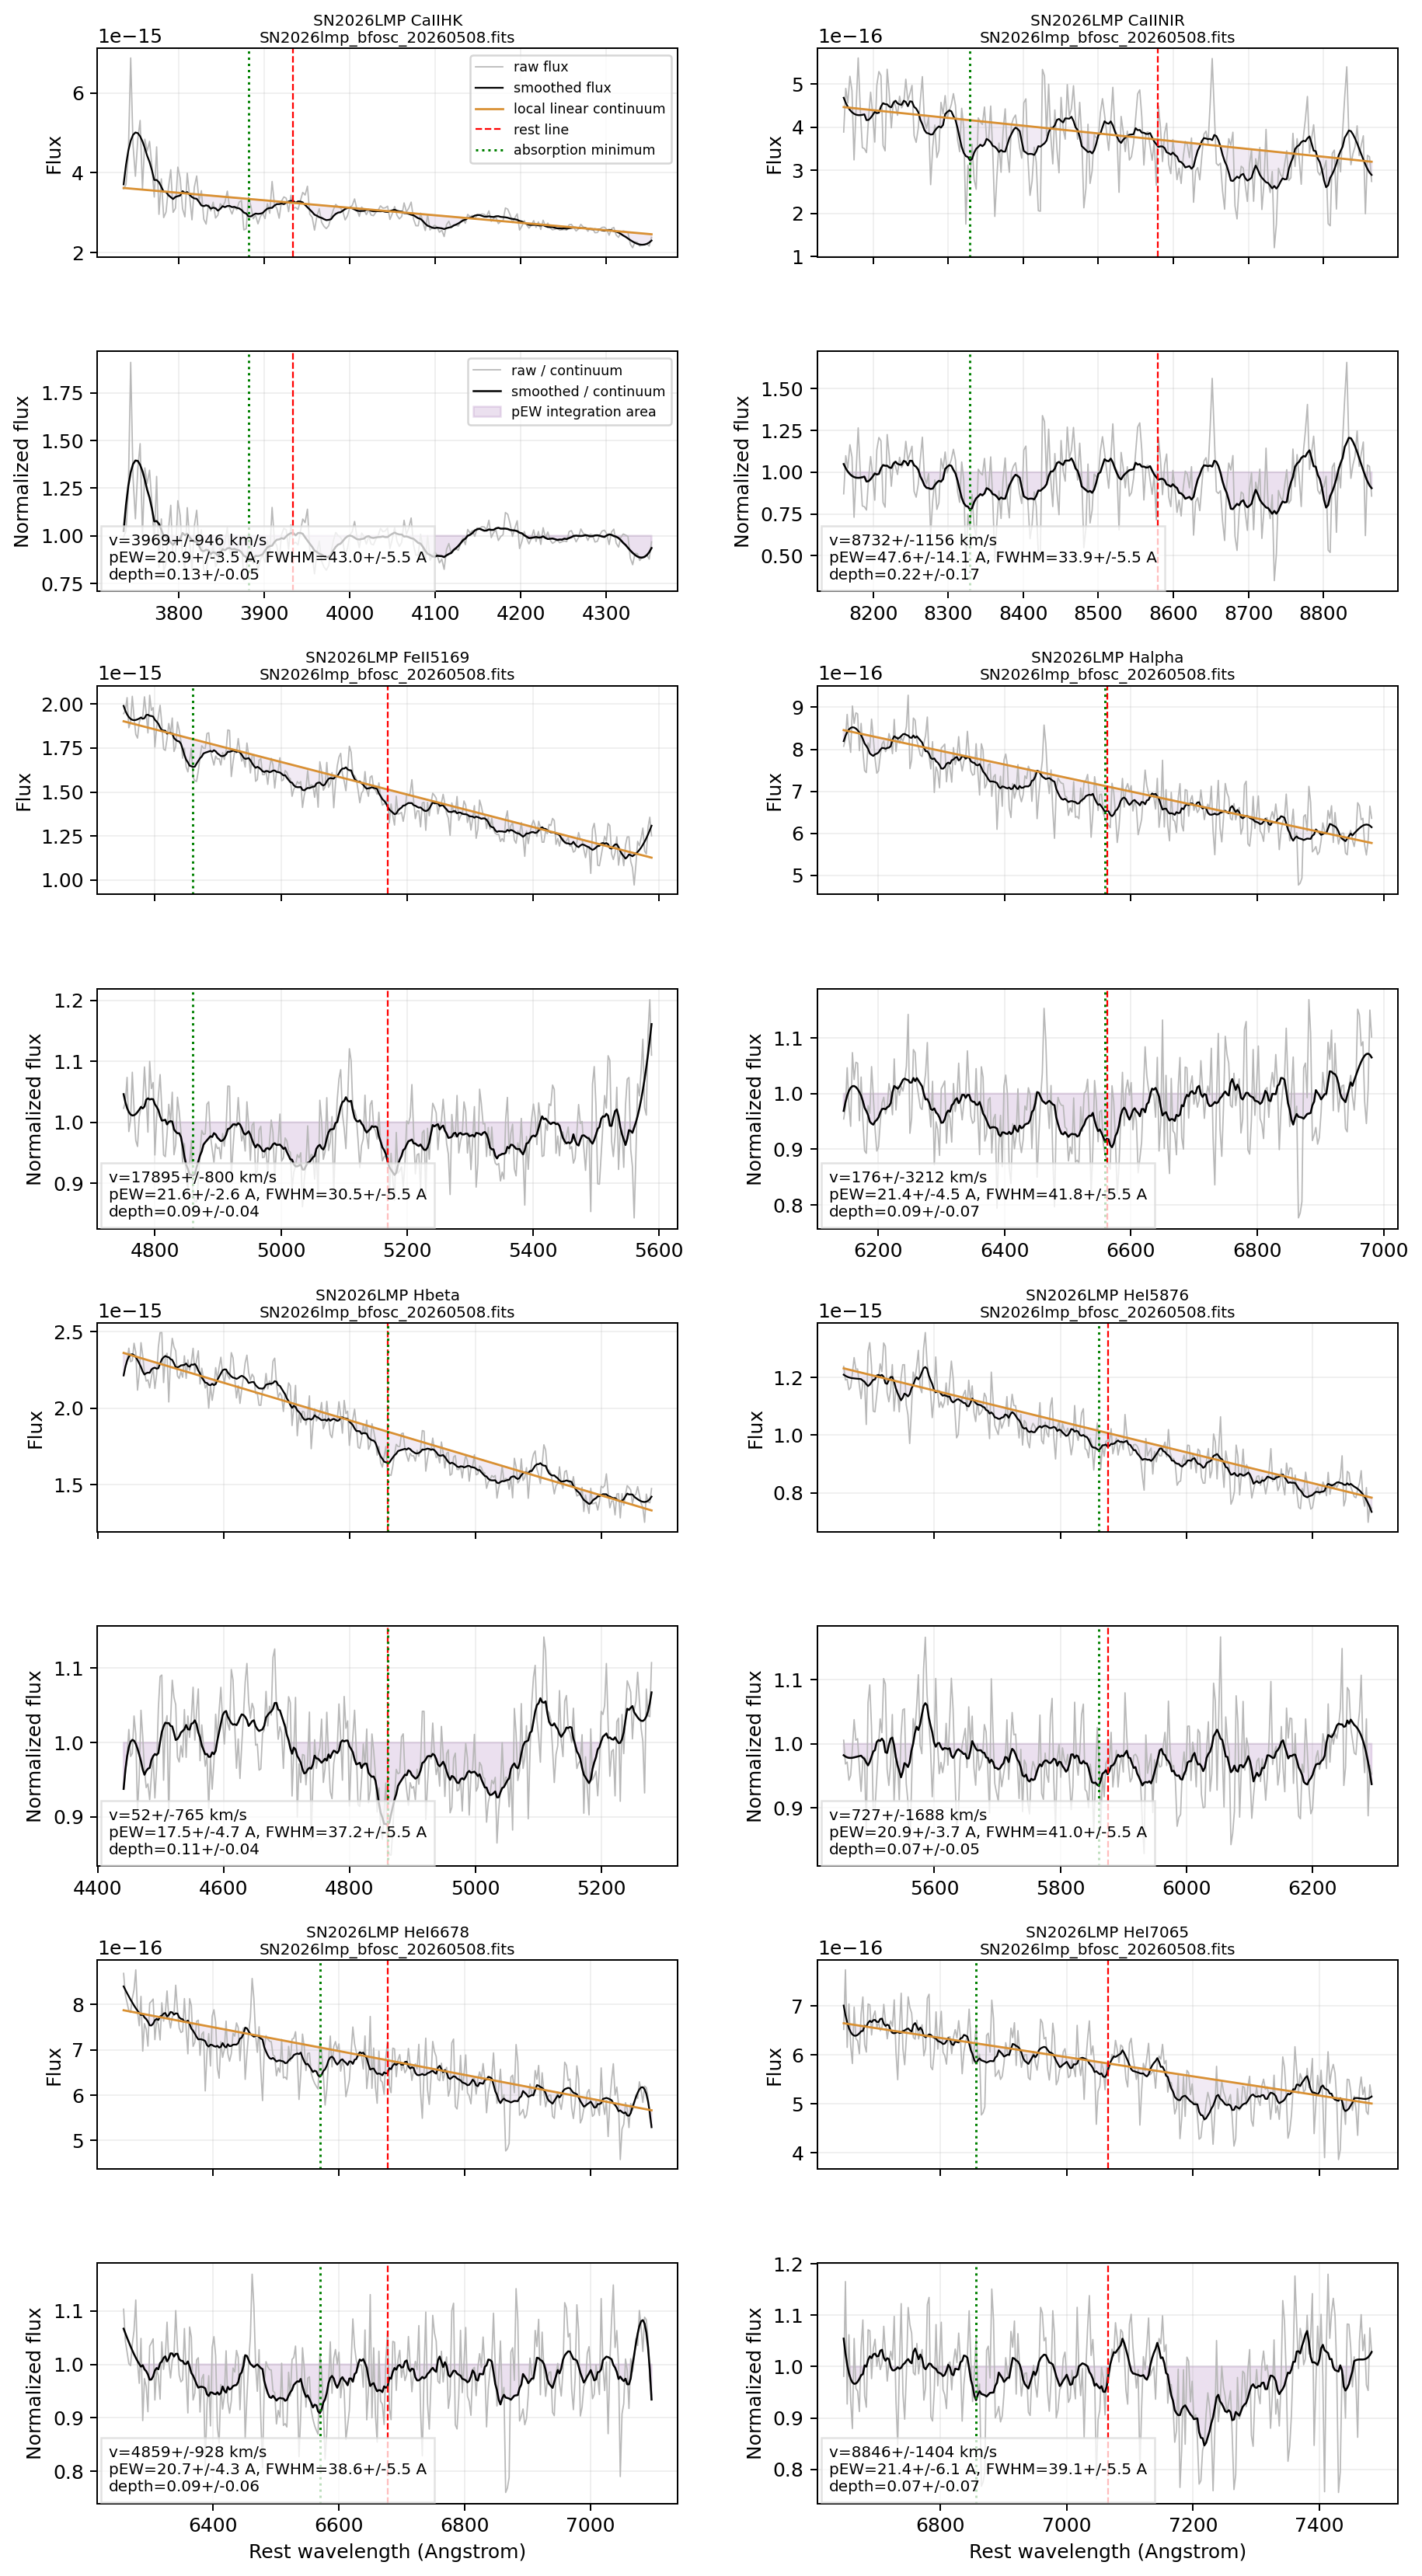
\includegraphics[width=0.96\linewidth,height=0.68\textheight,keepaspectratio]{images_zzzaurak/SN2026LMP_line_diagnostics_grid.png}
\caption{Candidate-line inspection plot for SN2026LMP. Because the target lacks a reliable TNS redshift, all candidate features are retained only for qualitative checks. From code by Ziheng Zhang.}
\label{fig:lmp-line-grid}
\end{figure}

\subsection{Final Key Line Measurements}
\subsubsection{SN2026FVX}
SN2026FVX is the Type Ia supernova with the longest temporal coverage in this sample. The Si II 6355 velocity decreases from about $1.45\times10^4~{\rm km~s^{-1}}$ to about $8.4\times10^3~{\rm km~s^{-1}}$, and Ca II H\&K decreases from about $1.63\times10^4~{\rm km~s^{-1}}$ to about $8.7\times10^3~{\rm km~s^{-1}}$. The automatic Ca II H\&K trough on 2026 March 26 is too narrow and is kept as \code{check}, not adopted.

\begin{table}[htbp]
\centering
\caption{Adopted line measurements for SN2026FVX. From code by Ziheng Zhang.}
\label{tab:fvx-lines}
\begin{tabular}{r l r r r r}
\toprule
Phase & Line & $v$ & pEW & FWHM & Depth \\
d & & km s$^{-1}$ & \AA & \AA & \\
\midrule
1.7 & CaIIHK & $16252\pm1467$ & $9.4\pm15.9$ & $45.2\pm5.5$ & 0.18 \\
20.7 & CaIIHK & $9736\pm418$ & $7.9\pm3.2$ & $36.7\pm5.5$ & 0.11 \\
51.6 & CaIIHK & $8742\pm732$ & $29.8\pm8.2$ & $47.0\pm5.5$ & 0.44 \\
1.7 & SiII6355 & $14550\pm843$ & $12.4\pm14.6$ & $60.4\pm5.5$ & 0.13 \\
8.7 & SiII6355 & $11004\pm324$ & $62.5\pm1.9$ & $126.0\pm5.5$ & 0.47 \\
20.7 & SiII6355 & $10237\pm324$ & $85.9\pm1.6$ & $128.6\pm5.5$ & 0.65 \\
51.6 & SiII6355 & $8441\pm324$ & $23.3\pm3.7$ & $58.4\pm5.5$ & 0.26 \\
\bottomrule
\end{tabular}
\end{table}

\subsubsection{SN2026JLM}
SN2026JLM is also a Type Ia supernova, but the observations are concentrated between about 14.5 and 26.6 days after discovery. The Si II 6355 velocity stays near $1.1\times10^4~{\rm km~s^{-1}}$ with no clear trend over this short phase range. The two adopted Ca II H\&K points suggest a decrease from a higher to a lower velocity, while the middle epoch is kept as \code{check}.

\begin{table}[htbp]
\centering
\caption{Adopted line measurements for SN2026JLM. From code by Ziheng Zhang.}
\label{tab:jlm-lines}
\begin{tabular}{r l r r r r}
\toprule
Phase & Line & $v$ & pEW & FWHM & Depth \\
d & & km s$^{-1}$ & \AA & \AA & \\
\midrule
14.5 & CaIIHK & $16017\pm413$ & $12.8\pm20.2$ & $24.7\pm5.4$ & 0.24 \\
26.6 & CaIIHK & $11526\pm310$ & $22.8\pm17.2$ & $51.7\pm5.4$ & 0.32 \\
14.5 & SiII6355 & $11410\pm768$ & $74.9\pm10.1$ & $138.2\pm5.4$ & 0.57 \\
22.5 & SiII6355 & $11242\pm832$ & $88.3\pm8.0$ & $146.3\pm5.4$ & 0.59 \\
26.6 & SiII6355 & $11337\pm512$ & $77.4\pm8.7$ & $139.6\pm5.4$ & 0.55 \\
\bottomrule
\end{tabular}
\end{table}

\subsubsection{SN2026KID}
SN2026KID is a Type II supernova. Fe II 5169 is used as the expansion-velocity scale indicator. The three epochs give velocities of roughly $0.8$--$1.1\times10^4~{\rm km~s^{-1}}$, but the uncertainties are large and the line depths are shallow, so the result should not be over-interpreted as a strictly monotonic evolution.

\begin{table}[htbp]
\centering
\caption{Adopted Fe II 5169 measurements for SN2026KID. From code by Ziheng Zhang.}
\label{tab:kid-lines}
\begin{tabular}{r l r r r r}
\toprule
Phase & Line & $v$ & pEW & FWHM & Depth \\
d & & km s$^{-1}$ & \AA & \AA & \\
\midrule
4.0 & FeII5169 & $11454\pm2714$ & $11.5\pm7.8$ & $85.7\pm5.5$ & 0.07 \\
5.0 & FeII5169 & $7723\pm1358$ & $11.5\pm8.5$ & $49.3\pm5.5$ & 0.10 \\
16.1 & FeII5169 & $8795\pm718$ & $18.7\pm7.7$ & $46.8\pm5.5$ & 0.16 \\
\bottomrule
\end{tabular}
\end{table}

\subsubsection{SN2026KIE and SN2026LMP}
SN2026KIE is a single-epoch SN Ic. Ca II H\&K and O I 7774 give a velocity scale of about $1.1\times10^4~{\rm km~s^{-1}}$, supporting a stripped-envelope interpretation. The Ca II NIR feature is shallow and has a large pEW uncertainty, so it is used only as supporting evidence. SN2026LMP is roughly consistent with a SN IIb classification, but it lacks a TNS redshift. All candidate lines are therefore retained only for qualitative checks and are not adopted as velocity, pEW, or FWHM measurements.

\begin{table}[htbp]
\centering
\caption{Single-epoch adopted line measurements for SN2026KIE. From code by Ziheng Zhang.}
\label{tab:kie-lines}
\begin{tabular}{r l r r r r}
\toprule
Phase & Line & $v$ & pEW & FWHM & Depth \\
d & & km s$^{-1}$ & \AA & \AA & \\
\midrule
16.3 & CaIIHK & $11287\pm418$ & $29.6\pm12.4$ & $25.6\pm5.5$ & 0.42 \\
16.3 & CaIINIR & $13799\pm672$ & $6.1\pm15.2$ & $43.3\pm5.5$ & 0.09 \\
16.3 & OI7774 & $11184\pm847$ & $15.7\pm13.8$ & $92.1\pm5.5$ & 0.17 \\
\bottomrule
\end{tabular}
\end{table}

\subsection{Evolution Figures and Auxiliary Diagnostics}
The following evolution figures show both \code{adopt} and \code{check} rows to preserve the manual-review trail. Quantitative conclusions use only the \code{adopt} measurements in the tables above. Faded or isolated \code{check} points, especially the no-redshift candidate features in SN2026LMP, are diagnostic only and are not used for velocity, pEW, or FWHM conclusions. Missing or very large error bars indicate substantial uncertainty from trough localization, local noise, or continuum-window choice.

\begin{figure}[htbp]
\centering
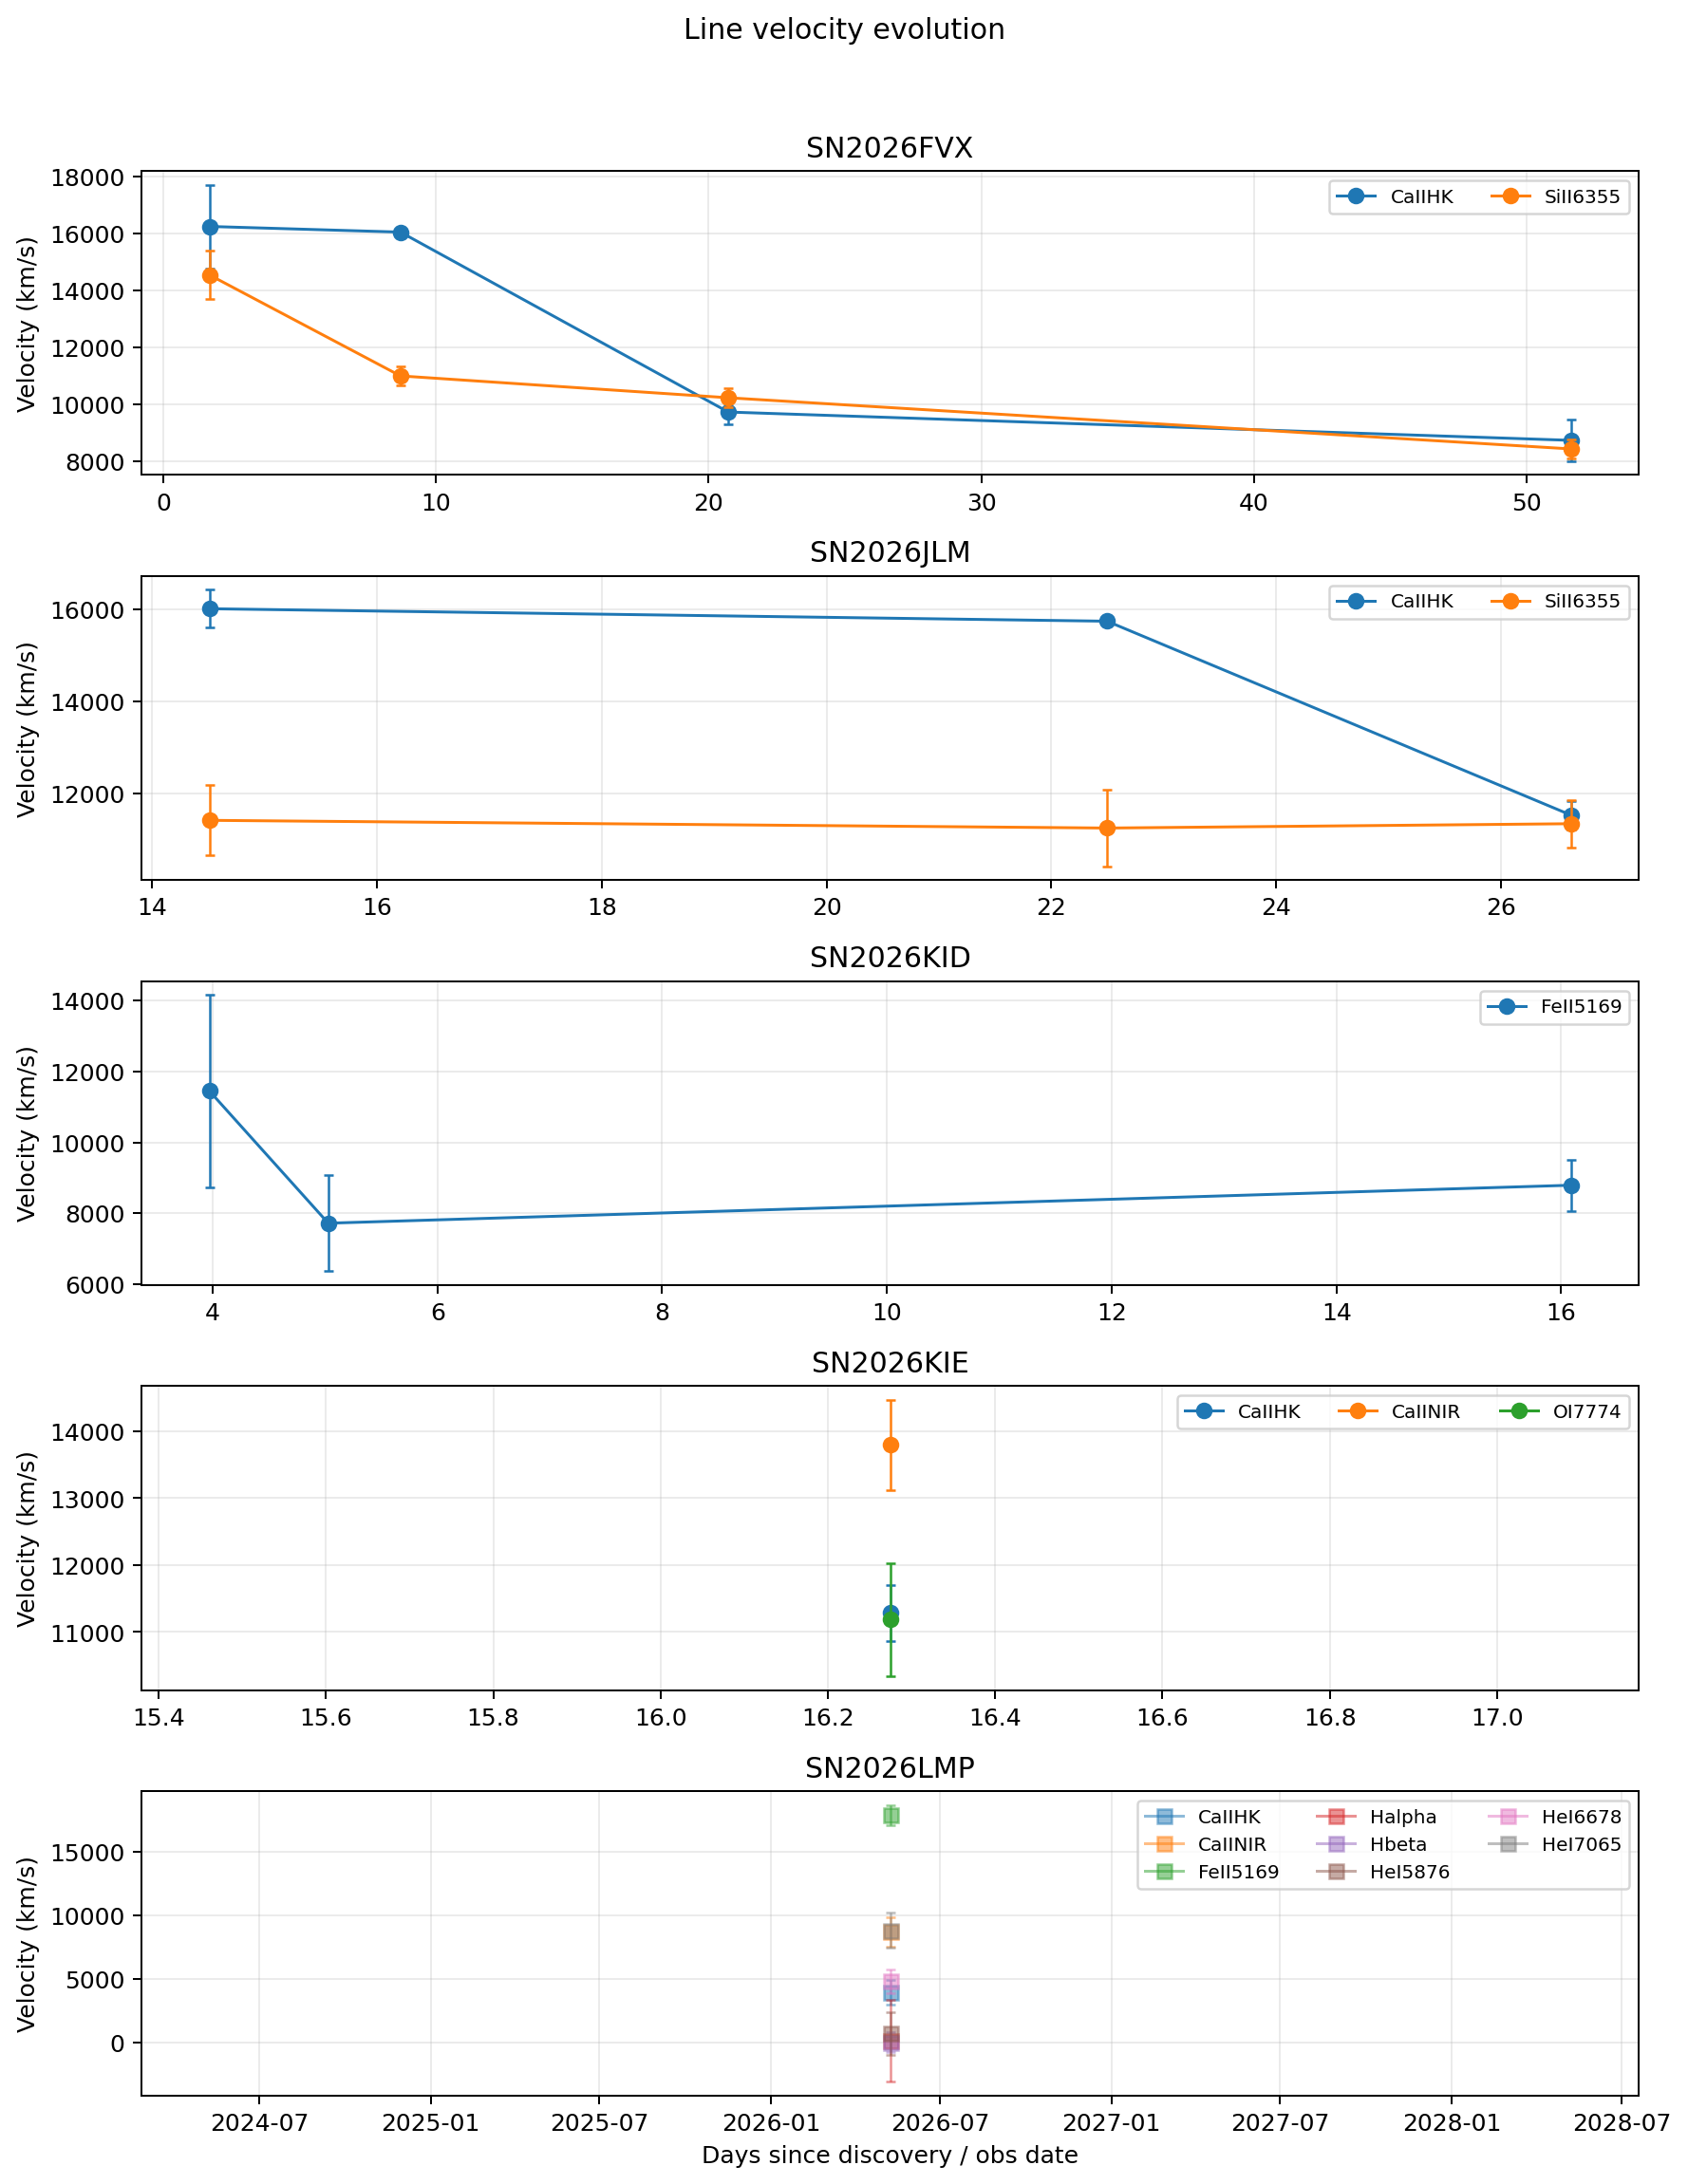
\includegraphics[width=0.95\linewidth]{images_zzzaurak/final5_line_velocity_evolution.png}
\caption{Line-velocity evolution as a function of days since discovery. The decline is clearest for Si II 6355 and Ca II H\&K in SN2026FVX, while Si II 6355 in SN2026JLM remains relatively stable over its shorter phase range. From code by Ziheng Zhang.}
\label{fig:velocity-evolution}
\end{figure}

\begin{figure}[htbp]
\centering
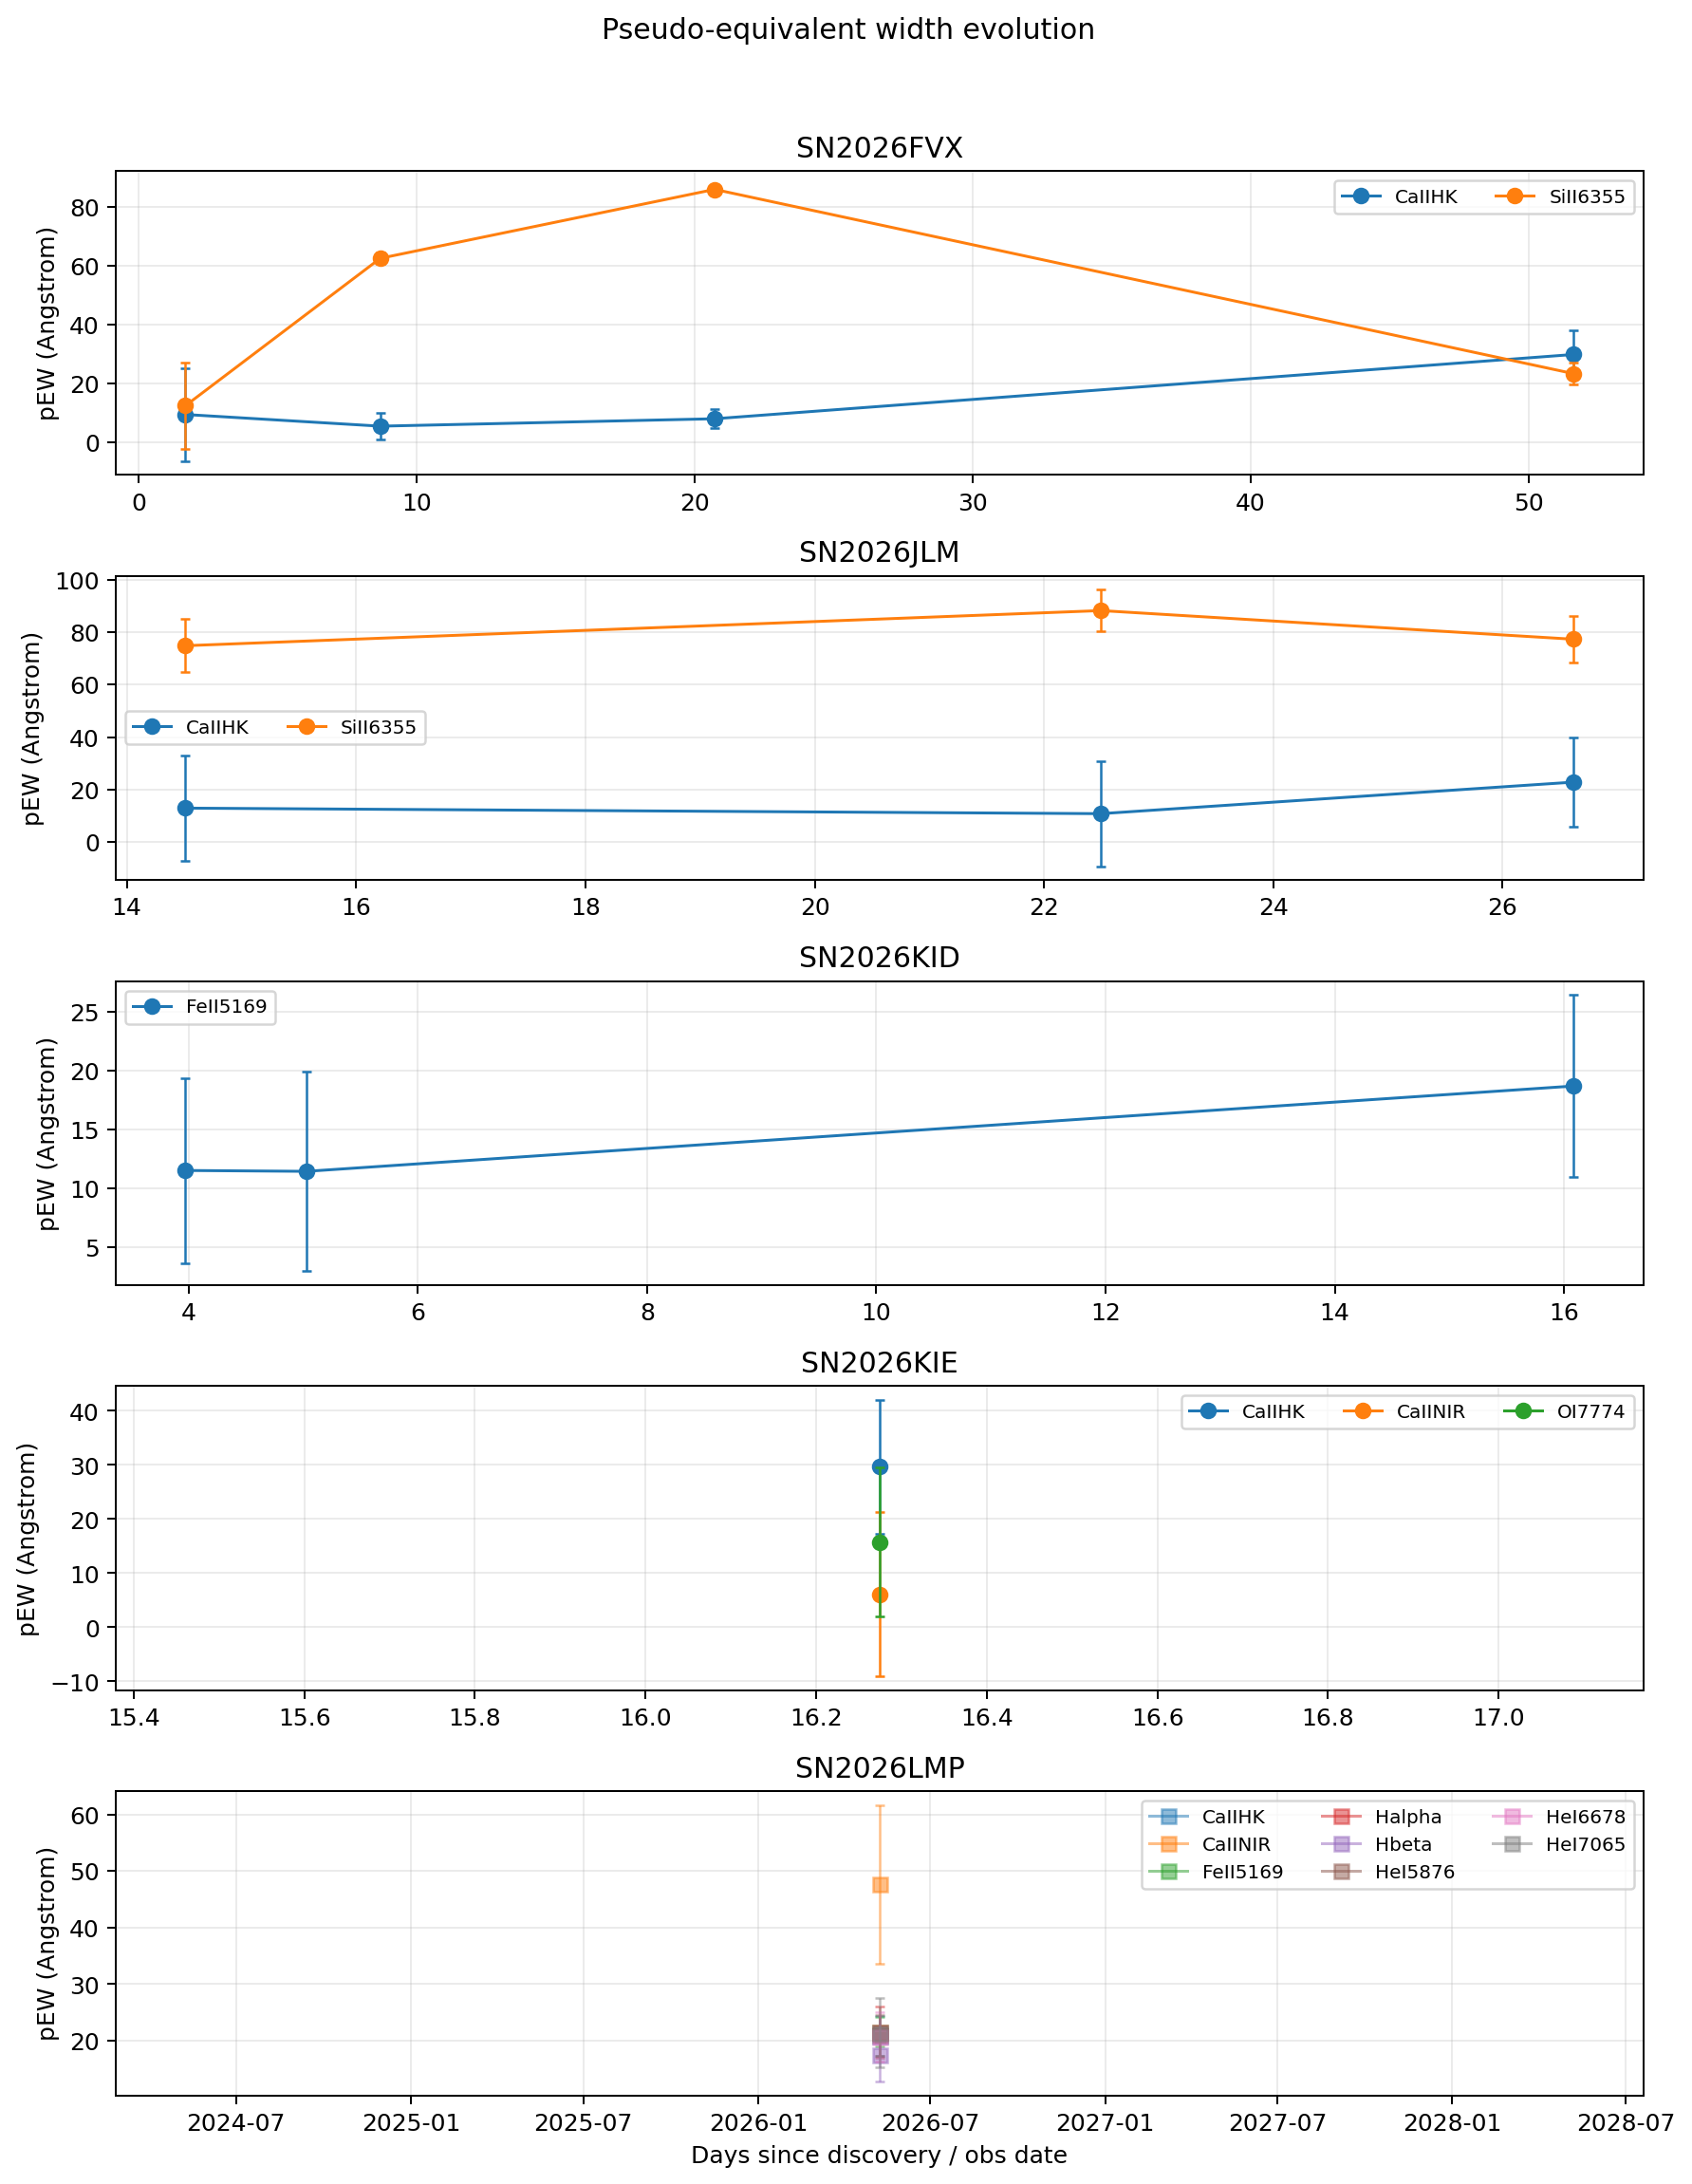
\includegraphics[width=0.95\linewidth]{images_zzzaurak/final5_pew_evolution.png}
\caption{Evolution of key-line pEW. The pEW is more sensitive to local-continuum placement and line blending, so weak lines or points with large uncertainties are used only as supporting information. From code by Ziheng Zhang.}
\label{fig:pew-evolution}
\end{figure}

\begin{figure}[htbp]
\centering
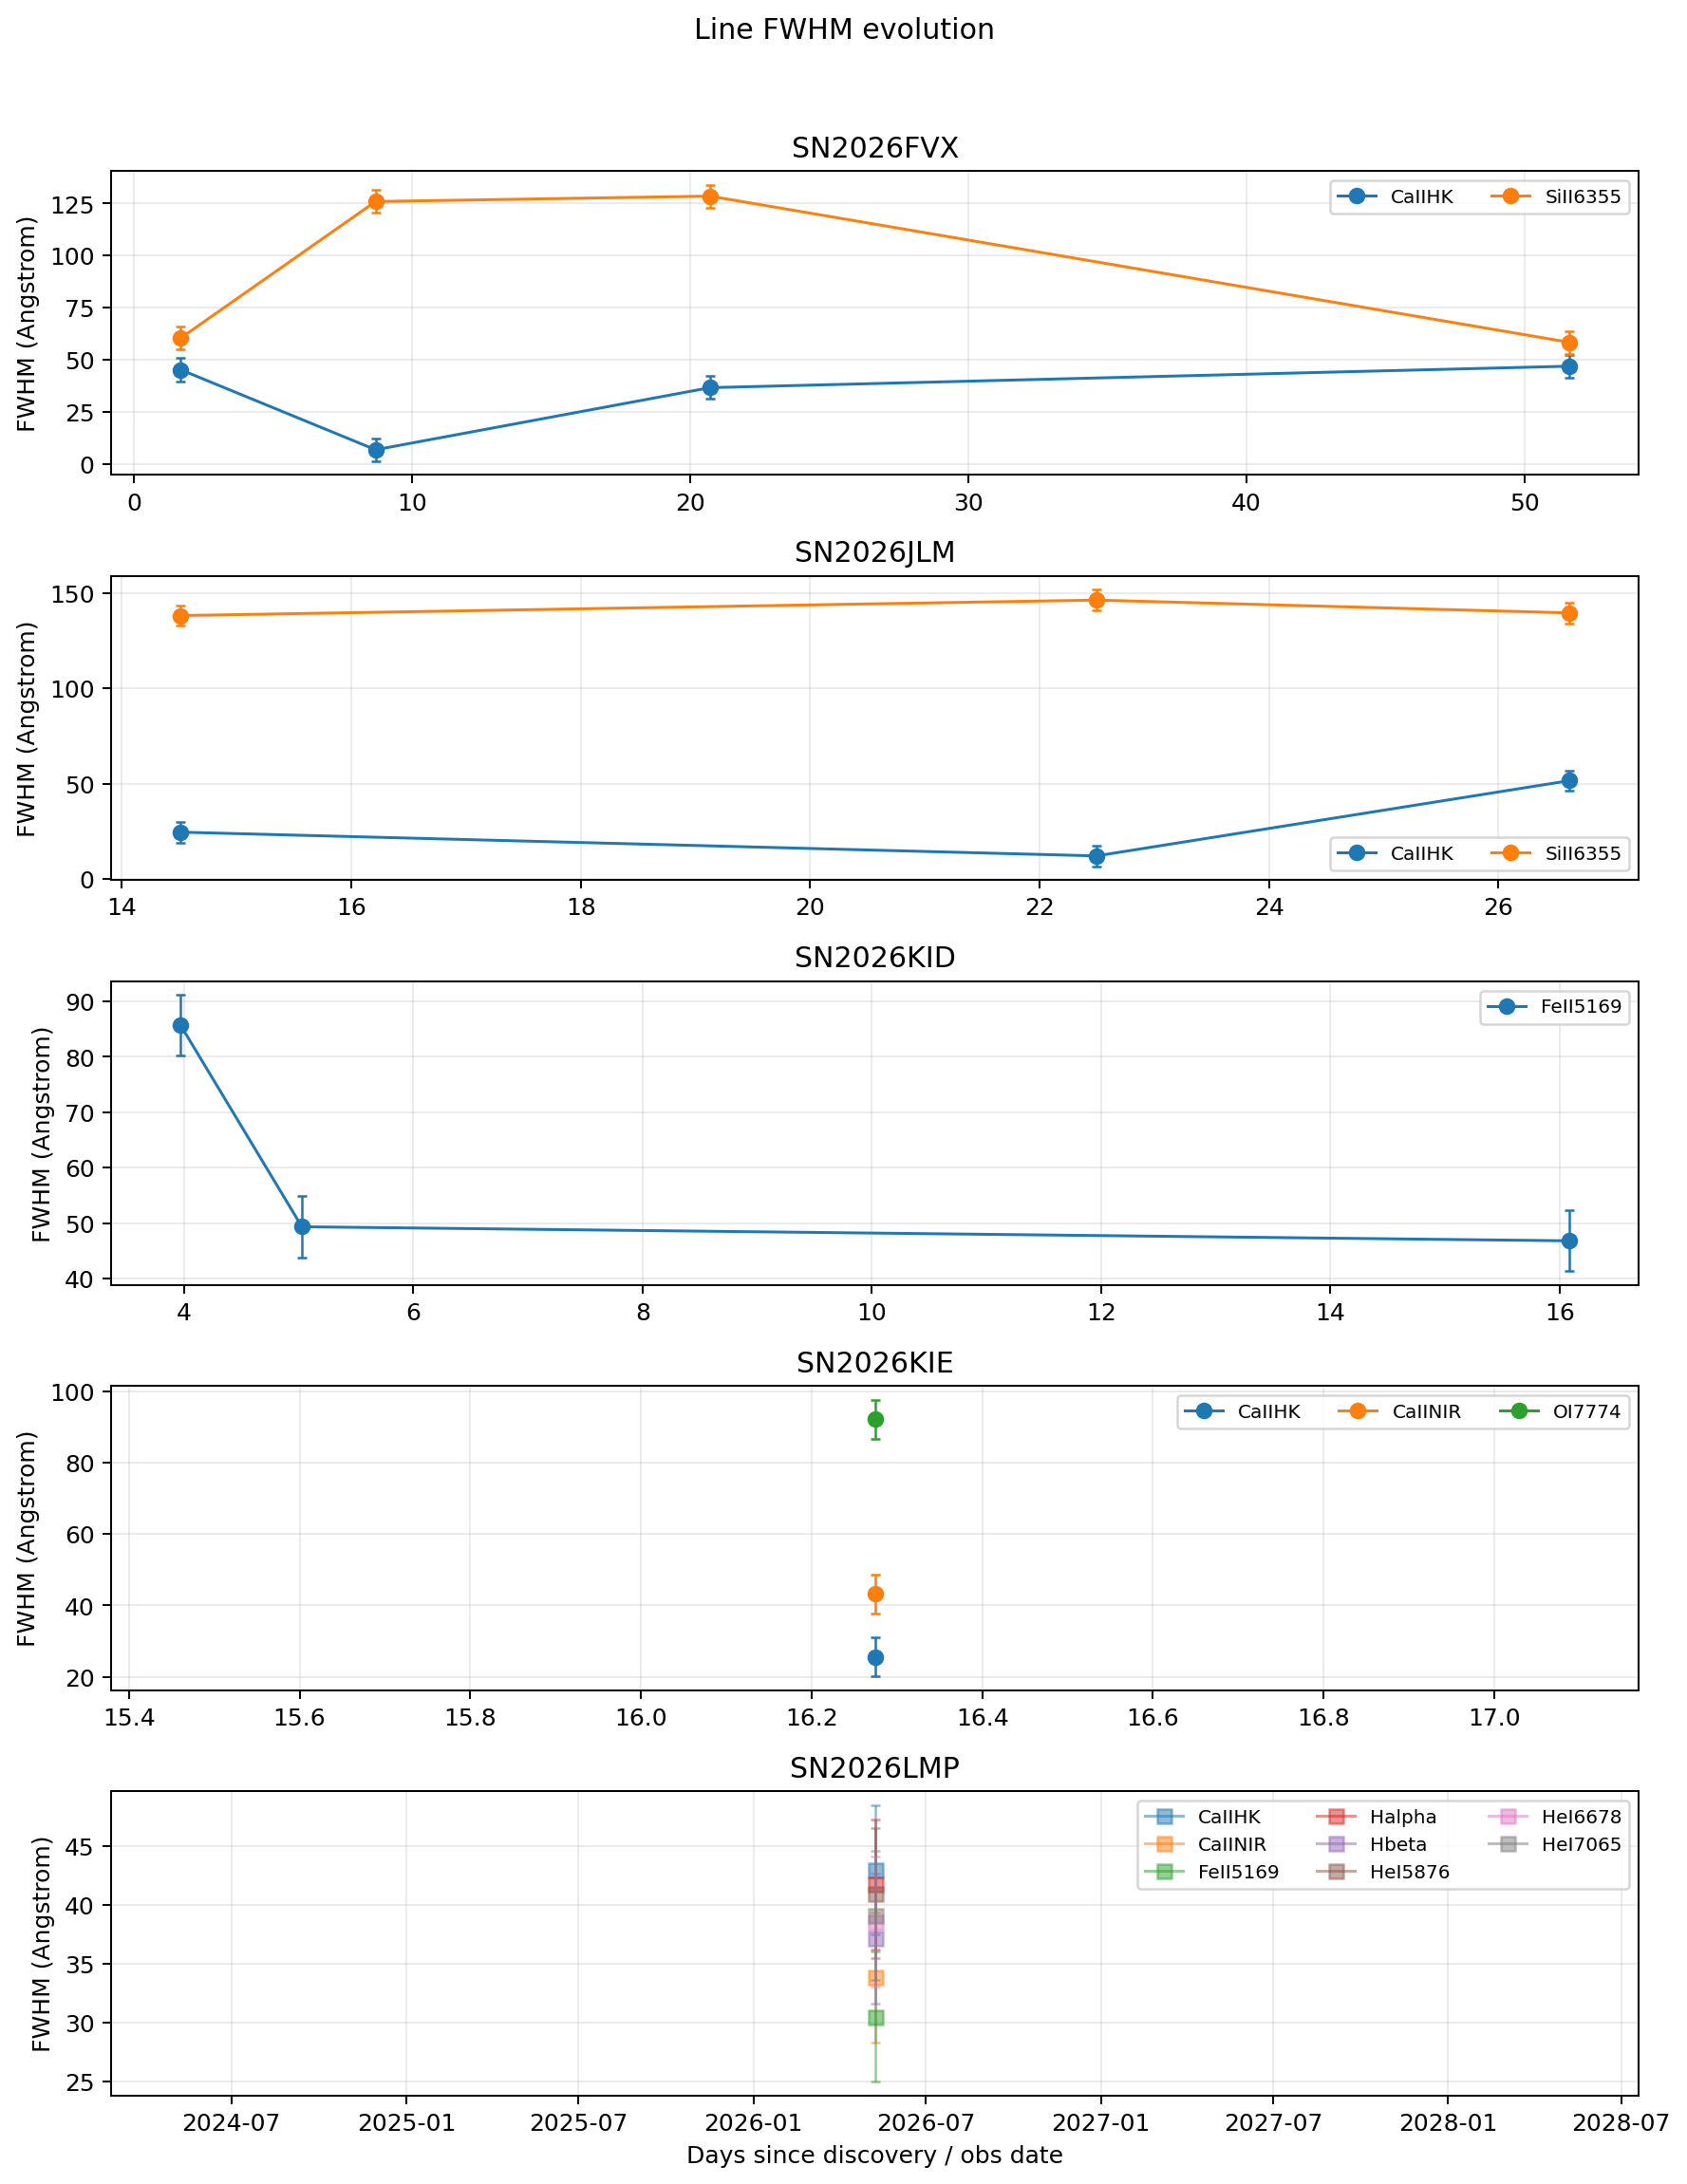
\includegraphics[width=0.95\linewidth]{images_zzzaurak/final5_fwhm_evolution.png}
\caption{Evolution of the non-parametric half-depth FWHM, measured from the half-depth crossings on either side of the trough minimum. From code by Ziheng Zhang.}
\label{fig:fwhm-evolution}
\end{figure}

\begin{figure}[htbp]
\centering
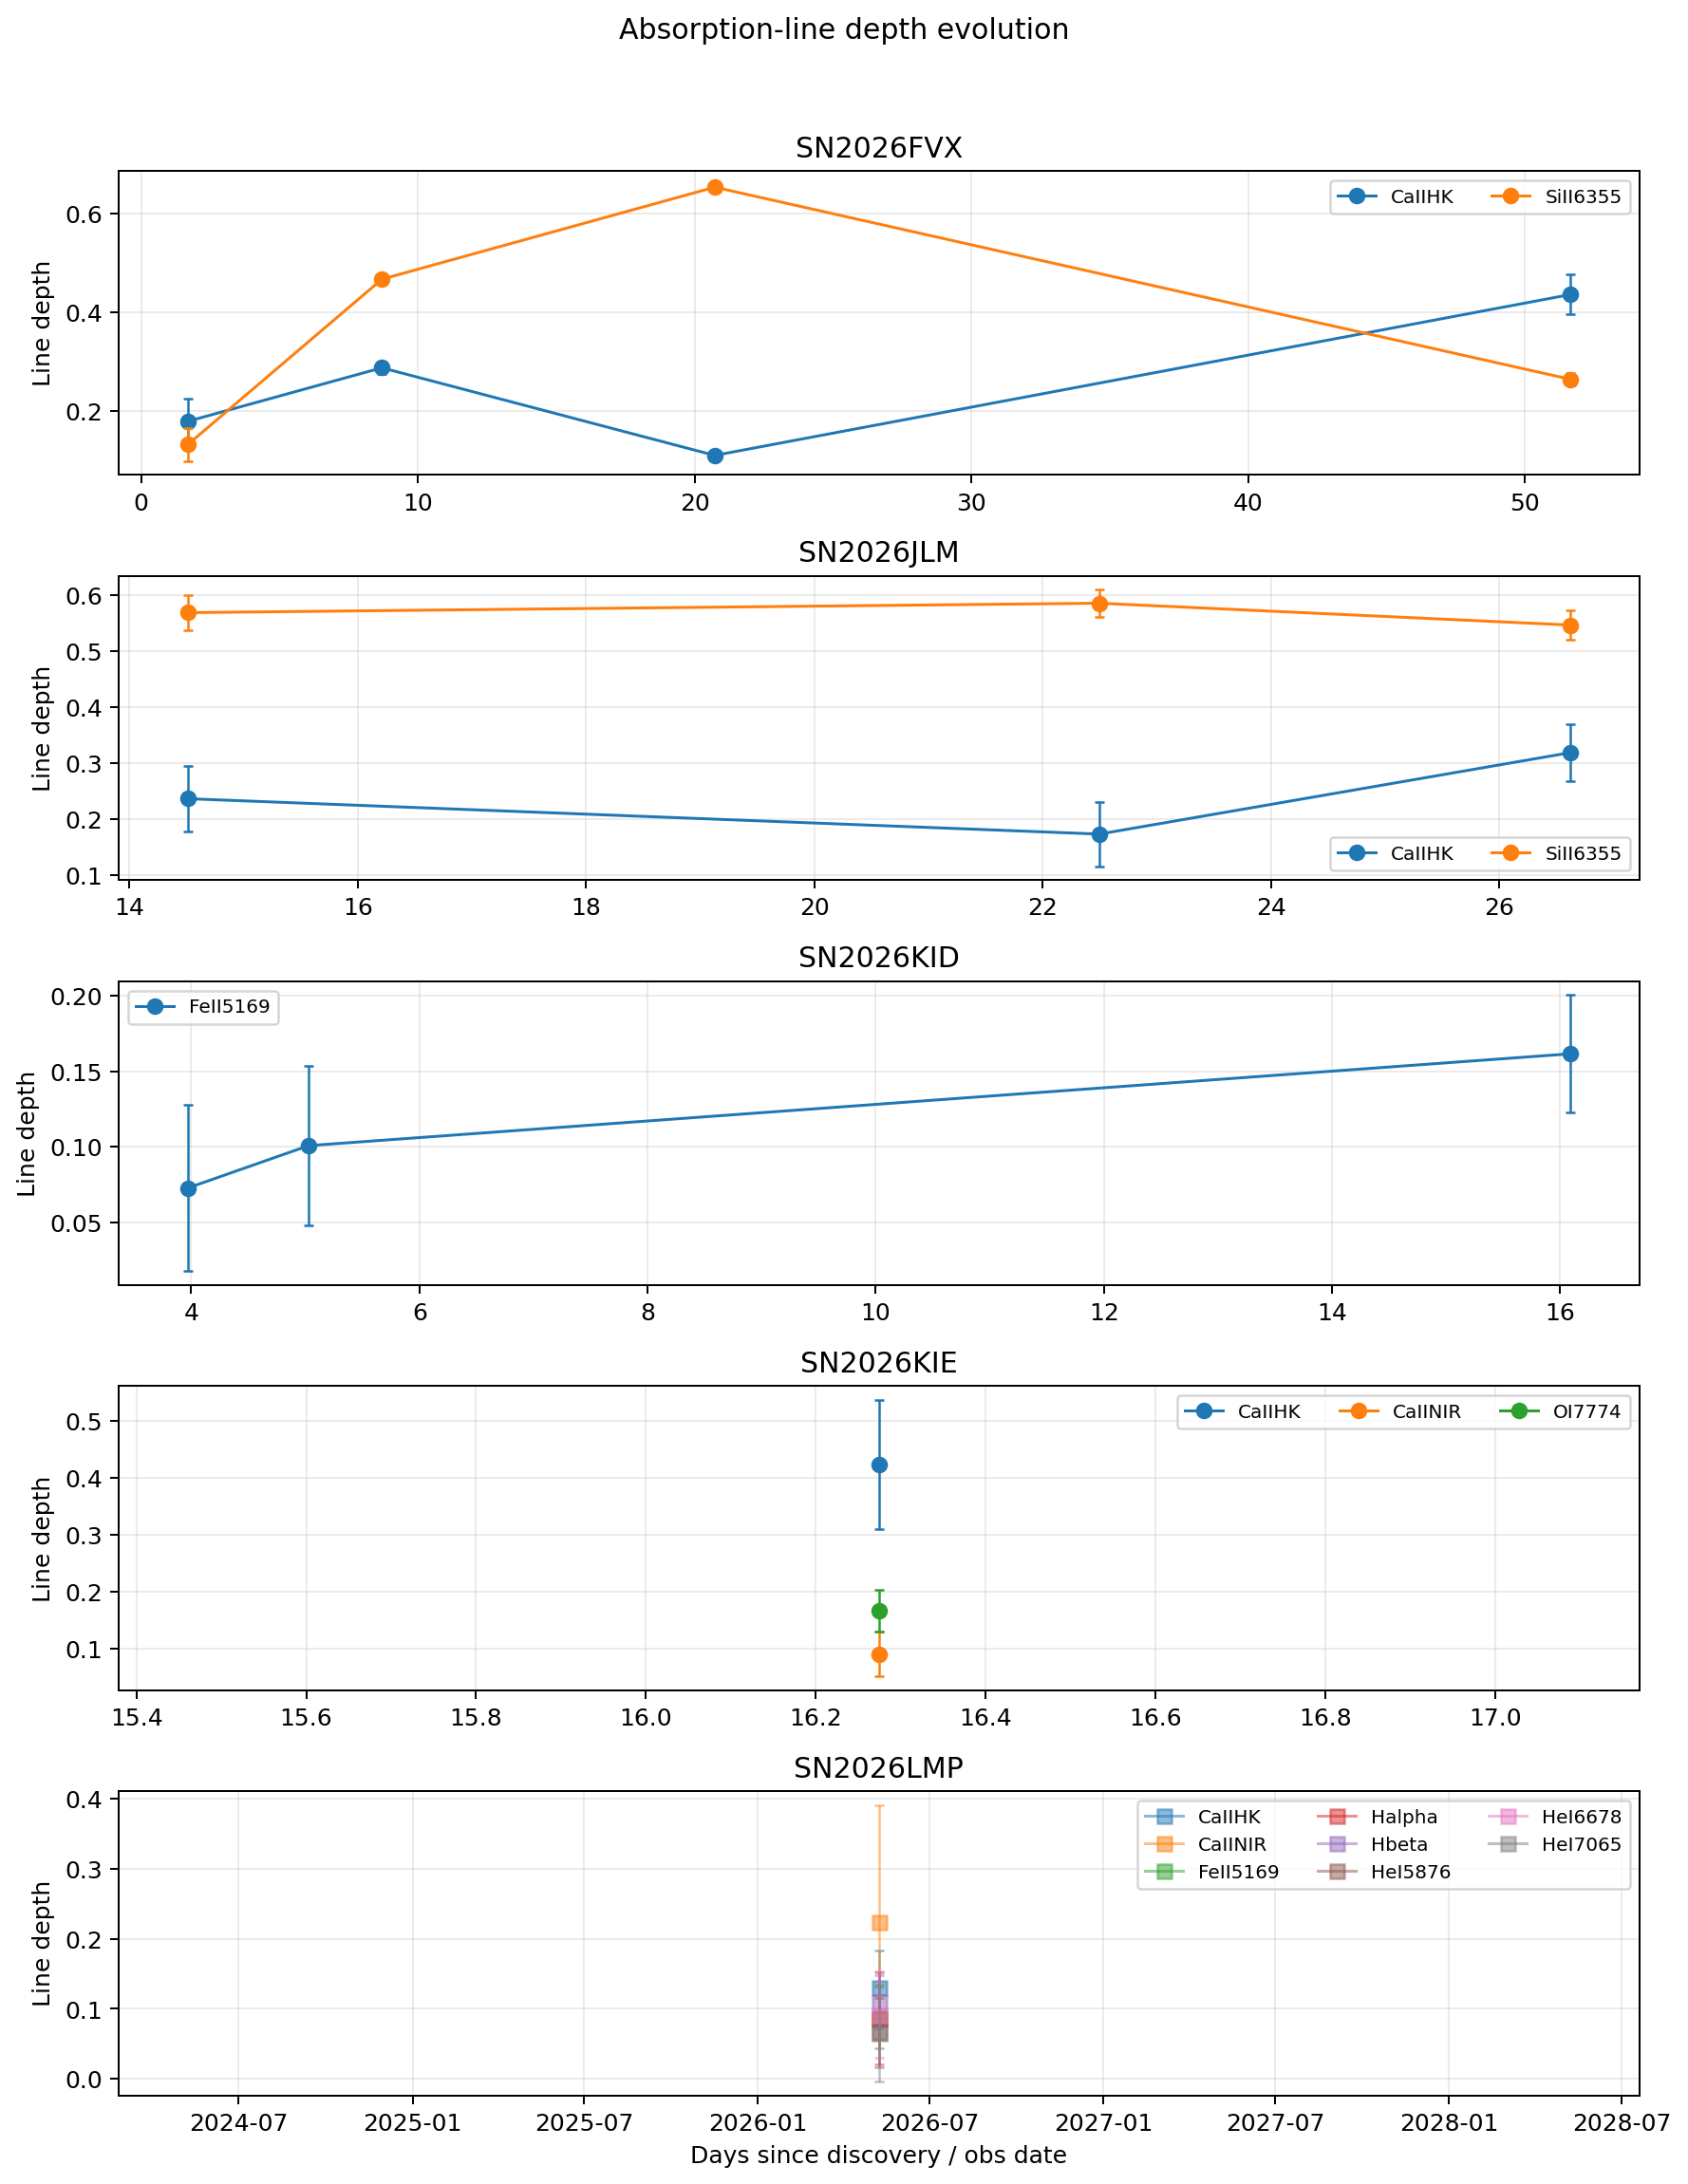
\includegraphics[width=0.95\linewidth]{images_zzzaurak/final5_line_depth_evolution.png}
\caption{Evolution of absorption-line depth. Shallow lines and points with large uncertainties should not be strongly over-interpreted. From code by Ziheng Zhang.}
\label{fig:depth-evolution}
\end{figure}

The blackbody color temperature is used only as a continuum-shape proxy. The horizontal axis in this evolution plot is \path{phase_days}. SN2026LMP does not have a phase relative to discovery, so it is not included in the evolution plot and is retained only in the CSV files and single-spectrum fit checks.

The blue-end spectral shape or redshift condition of SN2026KID, SN2026KIE, and SN2026LMP is not reliable enough for the temperature proxy to be a primary science conclusion.

\begin{figure}[htbp]
\centering
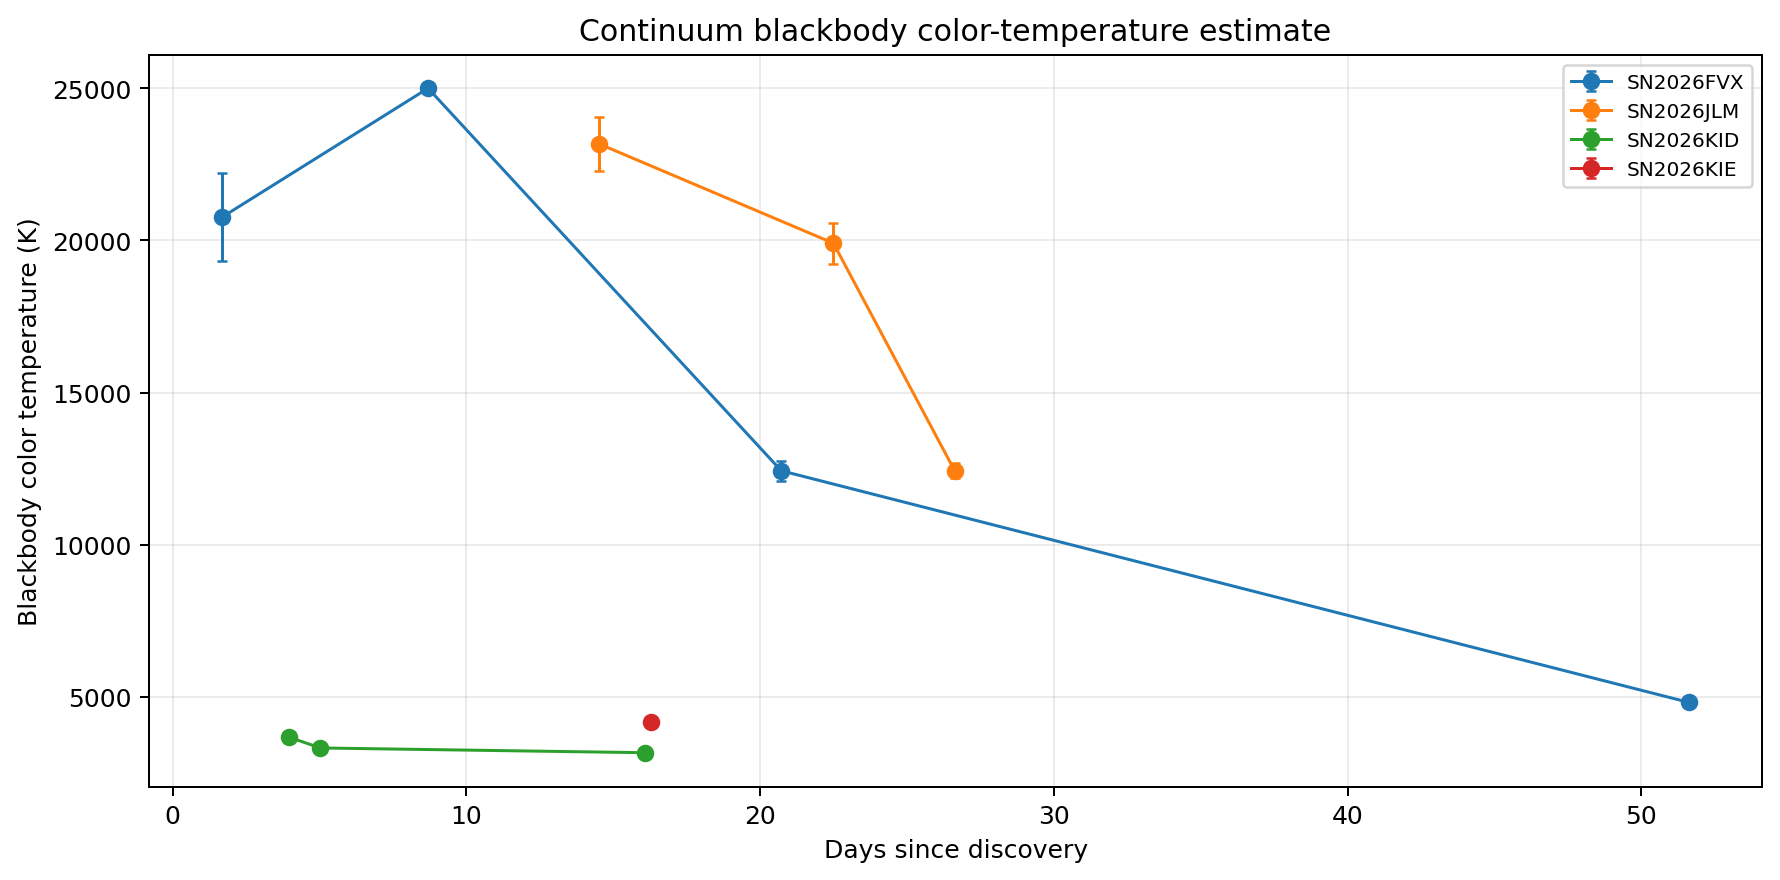
\includegraphics[width=0.95\linewidth]{images_zzzaurak/final5_blackbody_temperature.png}
\caption{Blackbody color-temperature proxy. This figure describes broad continuum-shape changes and is not a full radiative-transfer temperature measurement. From code by Ziheng Zhang.}
\label{fig:blackbody-temperature}
\end{figure}

\subsection{TARDIS Radiative-Transfer Modeling as Qualitative Support}
In addition to the empirical line measurements above, this section uses a set of one-dimensional Monte Carlo radiative-transfer simulations with TARDIS to check whether the main line identifications and velocity ranges are plausible. TARDIS is used here only as supporting evidence, not as the main evidence chain and not as a strict physical-parameter inversion. Because each supernova has only a few spectra and limited light-curve constraints, the model luminosity, time since explosion, velocity boundaries, density structure, and abundance presets are chosen to bring the synthetic spectrum close to the observed broad line positions and global spectral shape; they should not be interpreted directly as true ejecta mass, elemental abundance, or explosion energy.

The modeling does not fit every epoch. Instead, one representative early spectrum is selected for each supernova with a reliable redshift and classification. The four TARDIS targets are SN2026FVX, SN2026JLM, SN2026KID, and SN2026KIE. SN2026LMP is excluded from the quantitative TARDIS comparison because it lacks a reliable TNS redshift. The observed spectrum is shifted to the rest frame in the same way as above. Both simulated and observed spectra are smoothed and pseudo-continuum normalized before comparison, so the figures emphasize line positions and relative shape rather than absolute flux.

The candidate TARDIS parameters include total luminosity, time since explosion, velocity range, density profile, abundance preset, and plasma settings. The Type Ia targets use a W7-like \code{branch85\_w7} density structure. The Type II and Ibc targets use simplified \code{exponential} or \code{power\_law} density structures. The abundances are not fitted layer by layer, but are chosen from a small number of uniform presets, such as \code{ia\_standard}, \code{ia\_si\_rich}, \code{ii\_h\_rich}, and \code{ib\_he\_rich}. The model search also tests the Ia CSVY stratified model resources included with TARDIS and a more literature-like photospheric plasma preset, \code{nebular + dilute-lte + macroatom}. These more complex or more literature-like configurations do not automatically give better fits; the adopted models are still chosen by final-packet reruns and visual inspection.

The scoring function does not compare raw flux. Instead, it compares normalized spectral shape over the global overlap region and several diagnostic line windows. The total score combines broad RMSE, line-window RMSE, a correlation penalty, and absorption-trough position offsets; lower scores are closer under this normalization and line-window definition. The Type Ia windows emphasize Ca II H\&K, Si II 5972, Si II 6355, and Ca II NIR. The Type II windows emphasize H$\beta$, Fe II 5169, and H$\alpha$. The Ibc windows emphasize Ca II H\&K, Fe II 5169, O I 7774, and Ca II NIR.

\begin{table}[htbp]
\centering
\caption{Adopted TARDIS parameters for qualitative comparison. The score is used only for model screening under the same normalization and line-window definition; it should not be interpreted as a physical goodness ranking. From code by Ziheng Zhang.}
\label{tab:tardis-adopted}
\resizebox{\linewidth}{!}{%
\begin{tabular}{l l r r r l l l}
\toprule
Target & Candidate & Score & $\log L/L_\odot$ & Time (d) & Velocity range (km s$^{-1}$) & Density & Abundance preset \\
\midrule
SN2026FVX & \code{SN2026FVX\_c000} & 1.037 & 9.40 & 25.7 & 4374--13538 & \code{branch85\_w7} & \code{ia\_standard} \\
SN2026JLM & \code{SN2026JLM\_c001} & 1.753 & 9.40 & 32.5 & 5019--15534 & \code{branch85\_w7} & \code{ia\_si\_rich} \\
SN2026KID & \code{SN2026KID\_c002} & 1.136 & 8.80 & 25.0 & 5764--12488 & \code{exponential} & \code{ii\_h\_rich} \\
SN2026KIE & \code{SN2026KIE\_c000} & 1.287 & 9.00 & 31.3 & 8055--17452 & \code{power\_law} & \code{ib\_he\_rich} \\
\bottomrule
\end{tabular}}
\end{table}

For individual targets, the SN2026FVX Type Ia model is broadly aligned with the main Si II 6355 absorption and supports the Type Ia line identification, although the blue Ca II H\&K and Ca II NIR strengths still differ from the data. SN2026JLM also has a corresponding Si II 6355 structure, but the simulated absorption center is slightly too blue and Ca II NIR is too deep, so the comparison is qualitative only. SN2026KID gives the most stable TARDIS comparison among the four targets; the H$\alpha$ P-Cygni morphology and velocity range are reasonably consistent with the observed spectrum and provide a useful sanity check for the Type II interpretation. For SN2026KIE, the Ibc model partly reproduces the O I 7774 and Ca II NIR regions. Moving the adopted velocity range slightly to higher velocities reduces the overly deep 6200--6400~\AA\ absorption, but Ca II NIR remains too deep.

\begin{figure}[htbp]
\centering
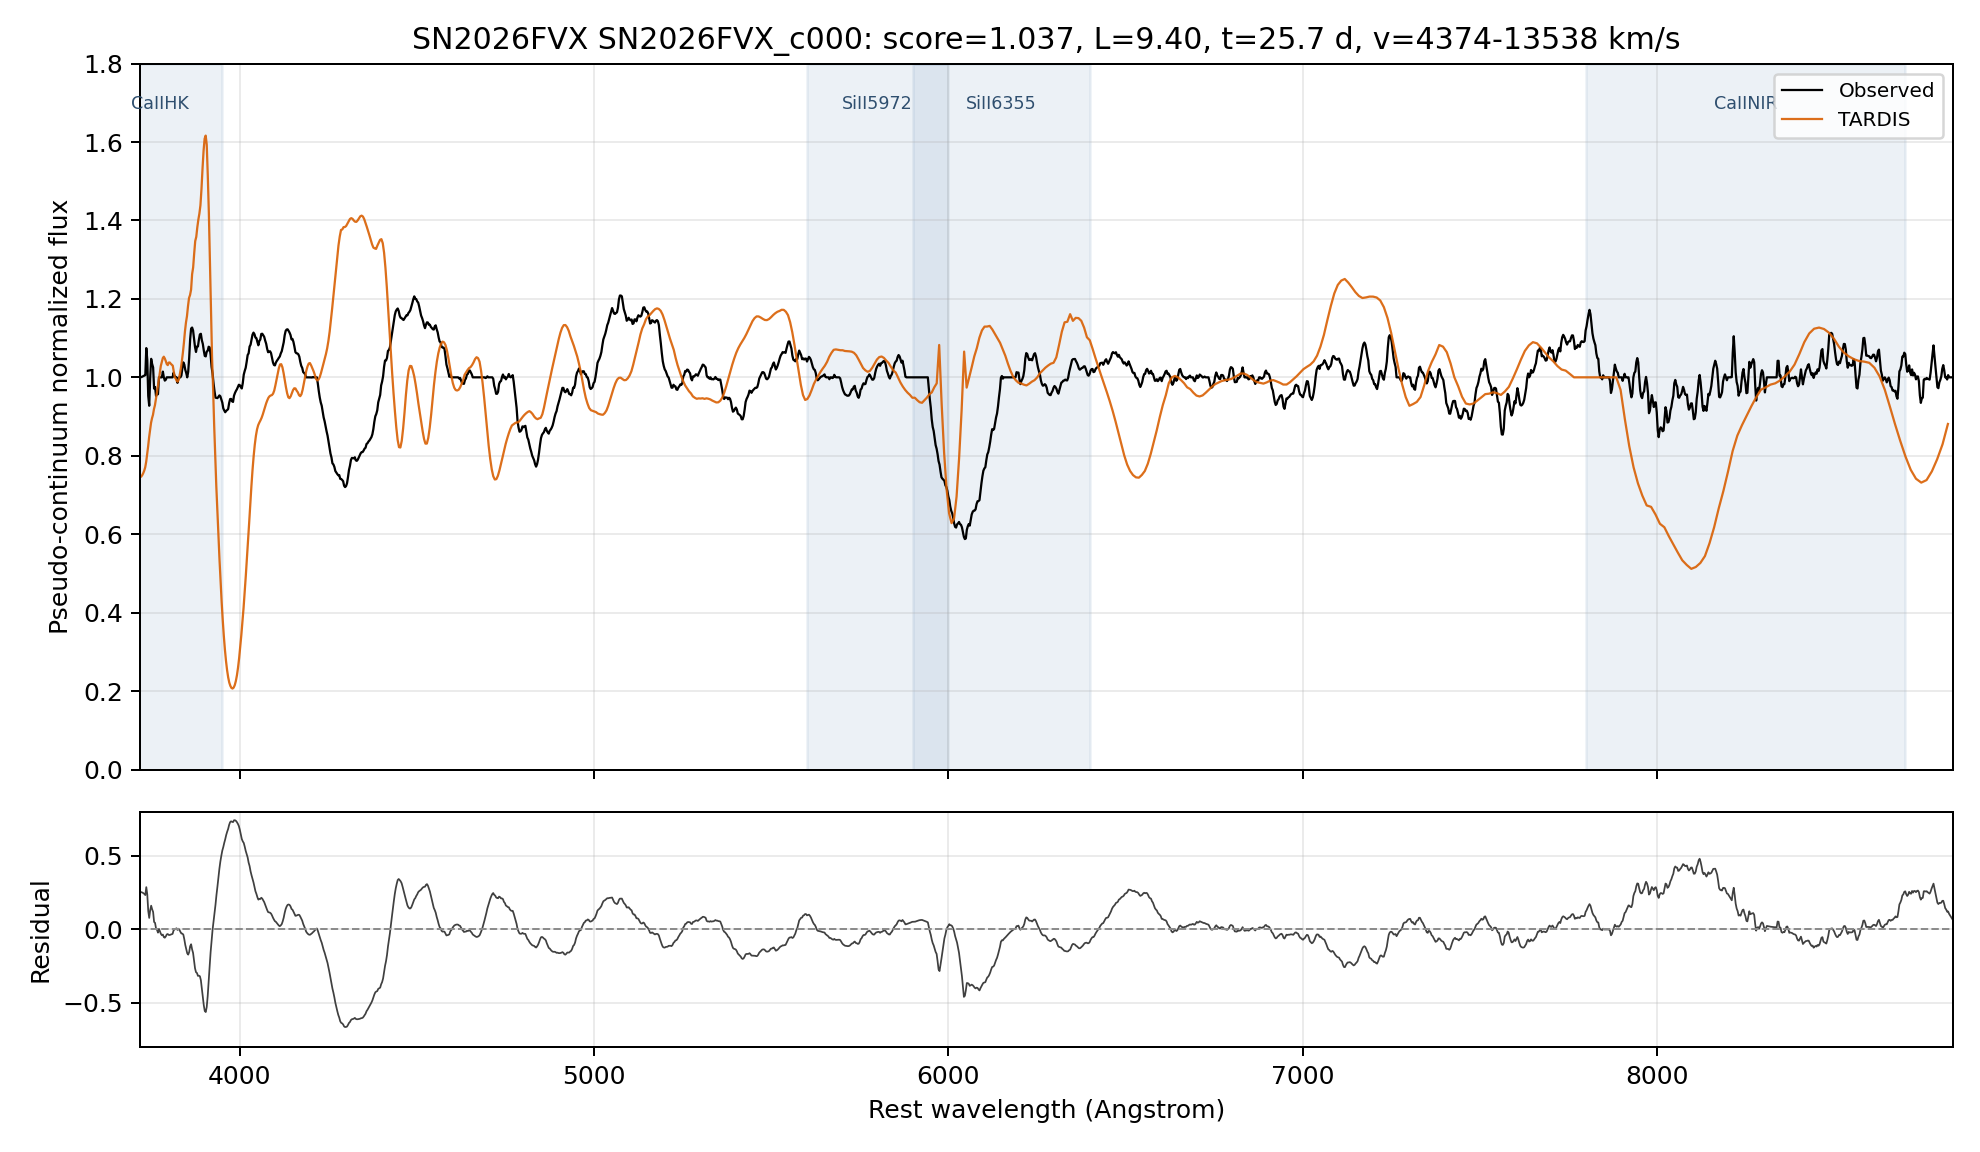
\includegraphics[width=0.95\linewidth]{images_zzzaurak/tardis_comparison_SN2026FVX.png}
\caption{Qualitative TARDIS comparison for SN2026FVX. The model mainly checks the line positions near Si II 6355 and the Ca II regions. From code by Ziheng Zhang.}
\label{fig:tardis-fvx}
\end{figure}

\begin{figure}[htbp]
\centering
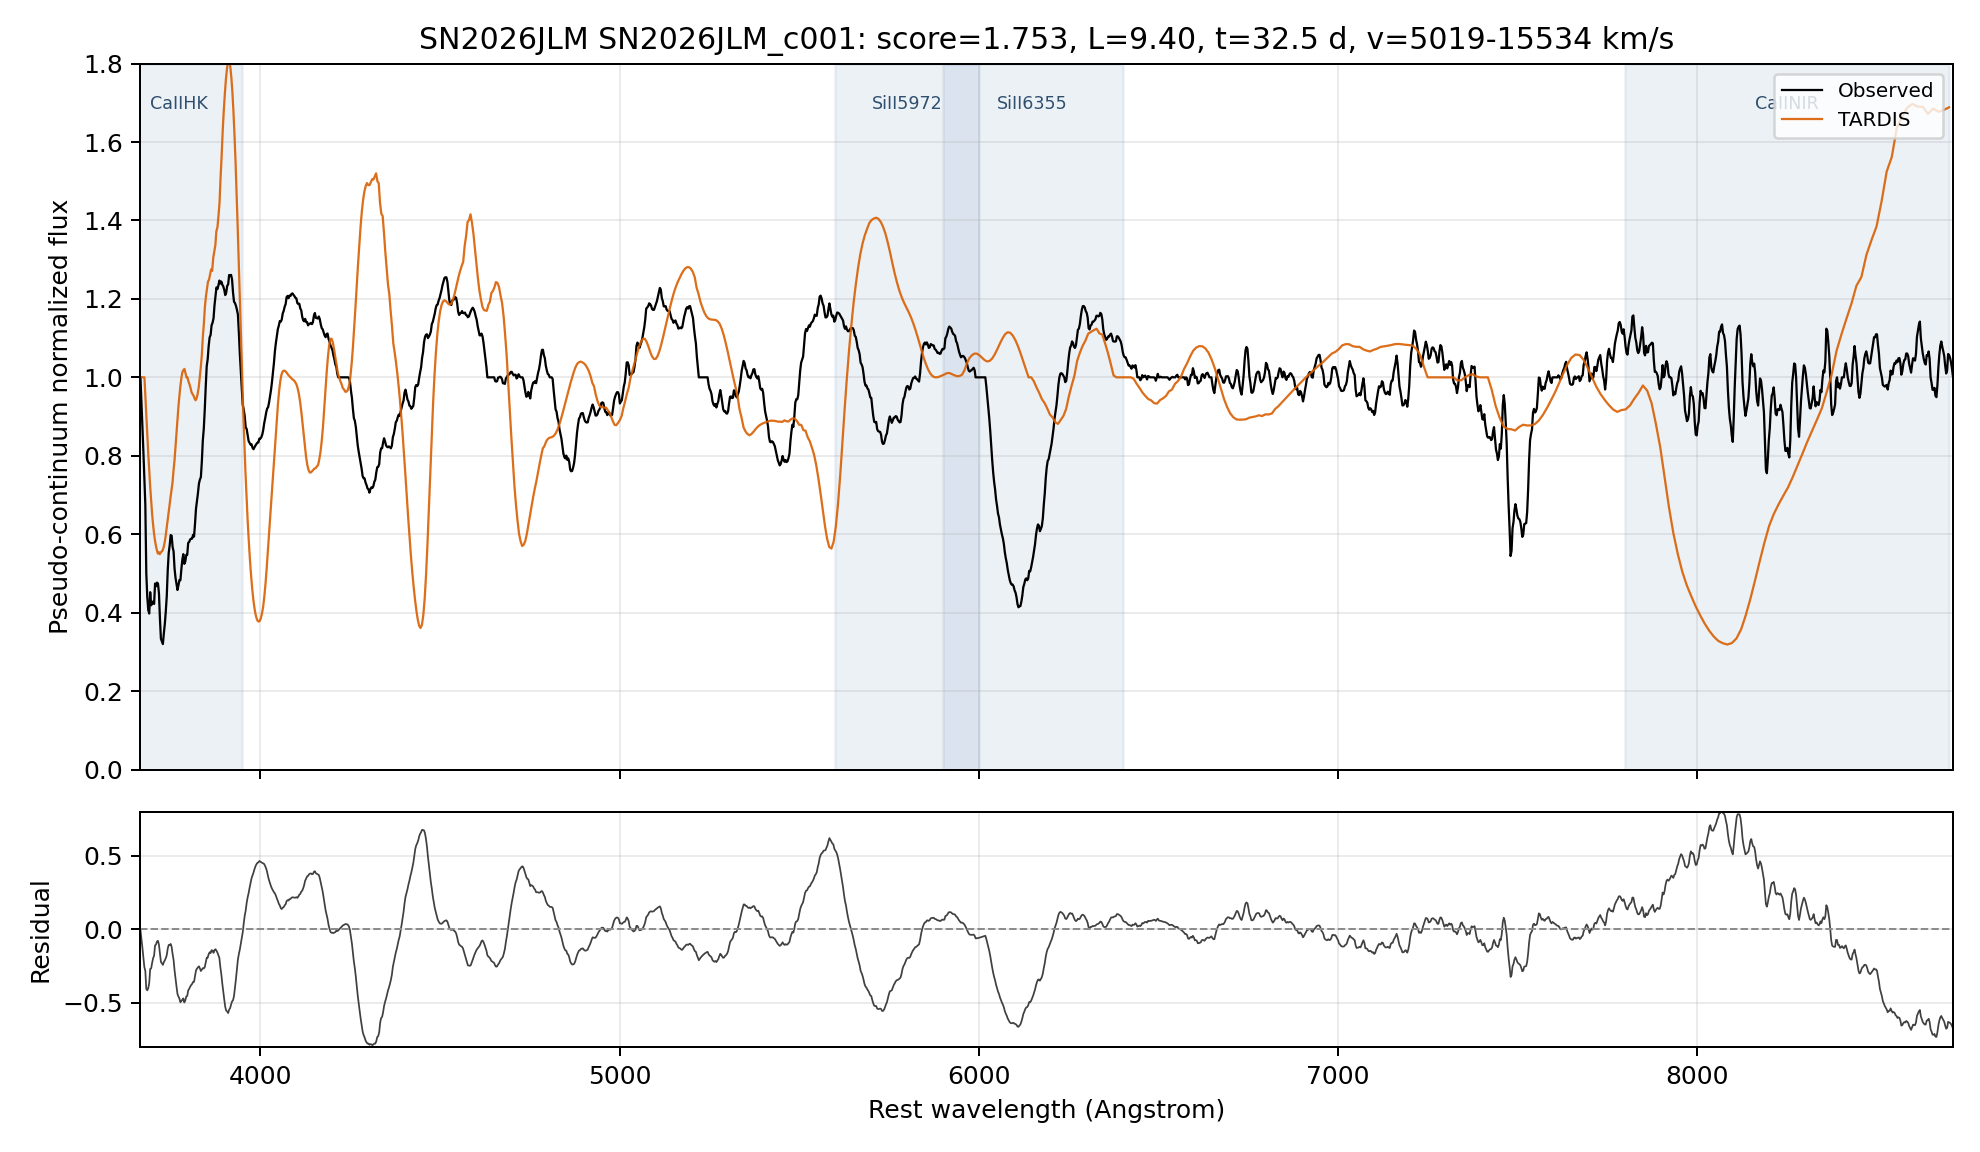
\includegraphics[width=0.95\linewidth]{images_zzzaurak/tardis_comparison_SN2026JLM.png}
\caption{Qualitative TARDIS comparison for SN2026JLM. The plot supports the Type Ia line identification but does not provide an abundance or explosion-parameter inversion. From code by Ziheng Zhang.}
\label{fig:tardis-jlm}
\end{figure}

\begin{figure}[htbp]
\centering
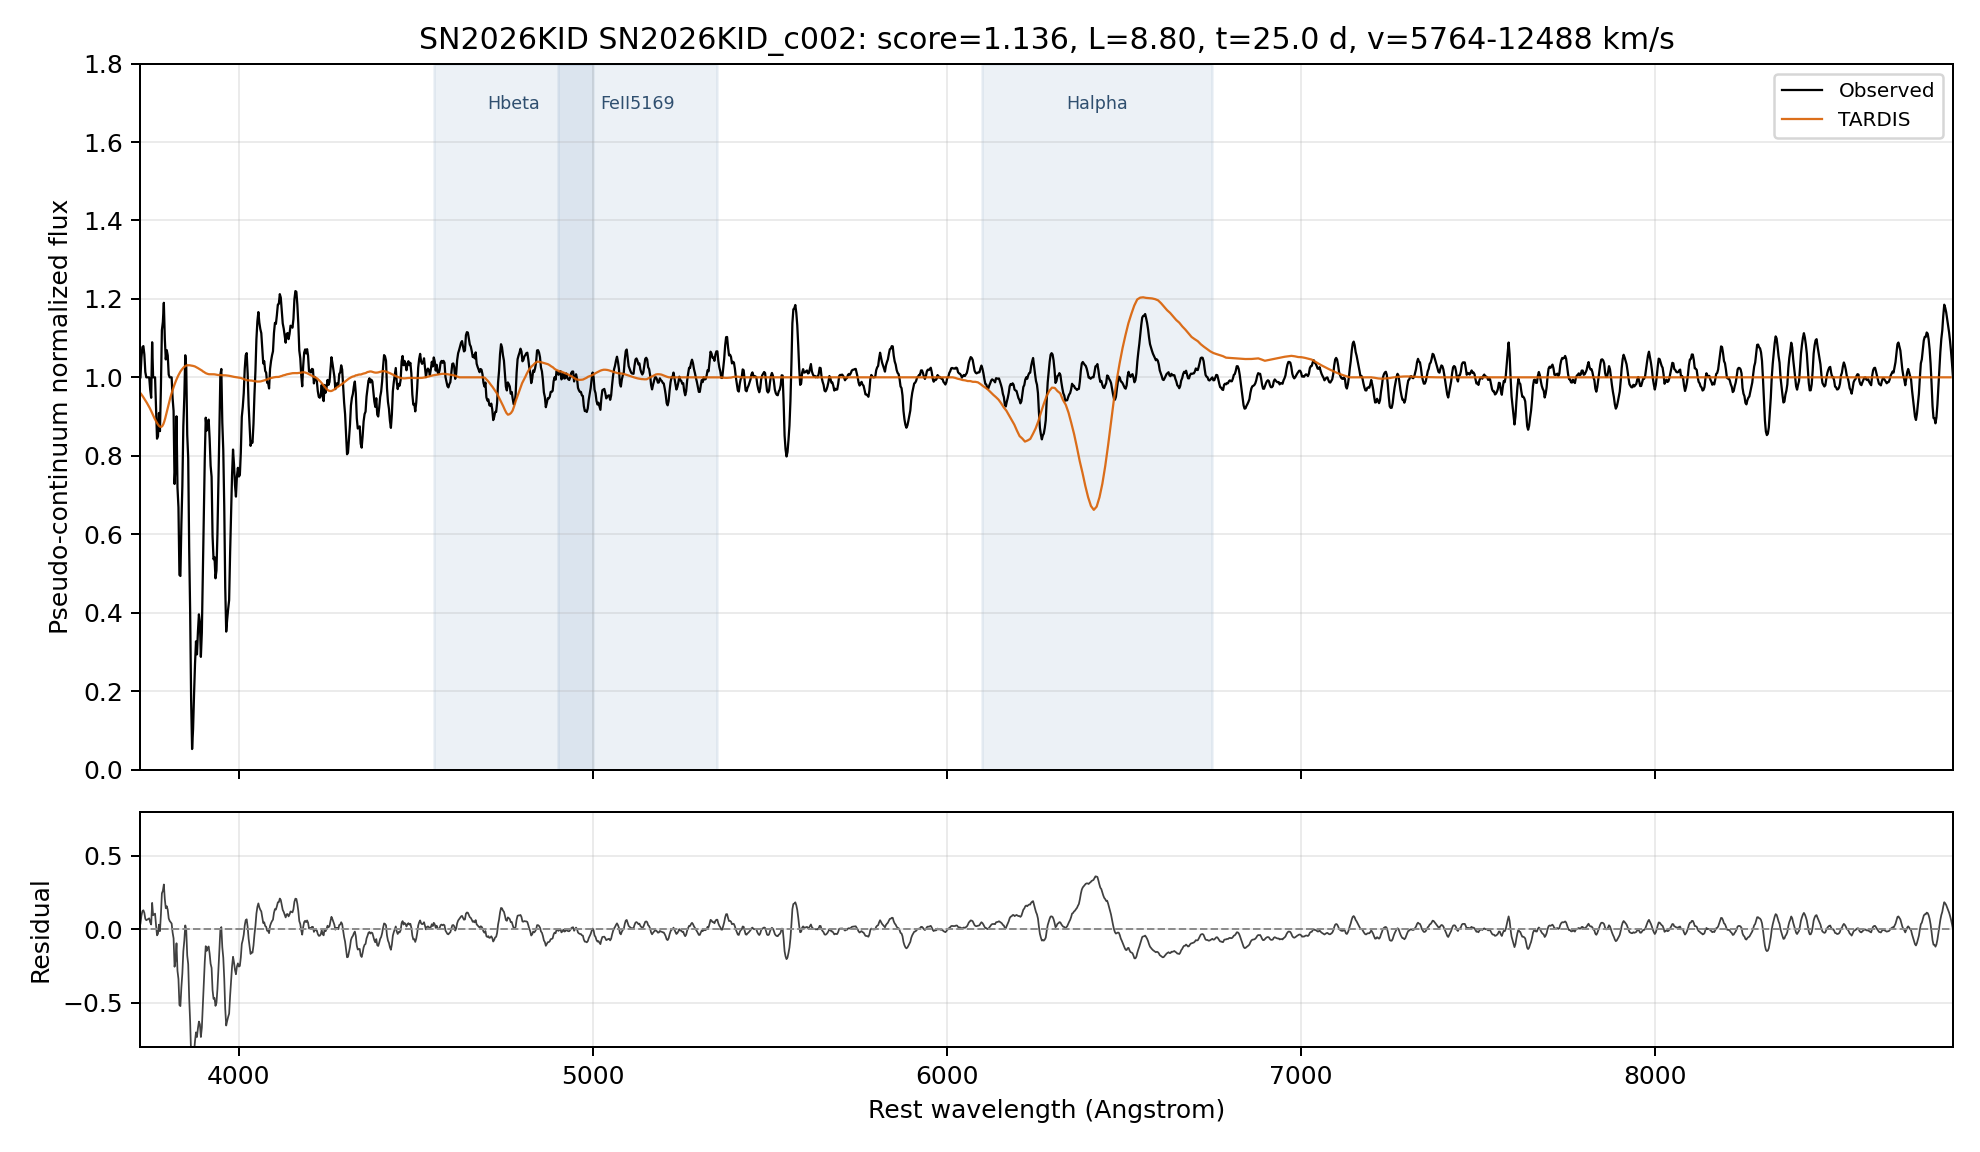
\includegraphics[width=0.95\linewidth]{images_zzzaurak/tardis_comparison_SN2026KID.png}
\caption{Qualitative TARDIS comparison for SN2026KID. The H$\alpha$ P-Cygni morphology is reasonably consistent with the observation and supports the Type II interpretation. From code by Ziheng Zhang.}
\label{fig:tardis-kid}
\end{figure}

\begin{figure}[htbp]
\centering
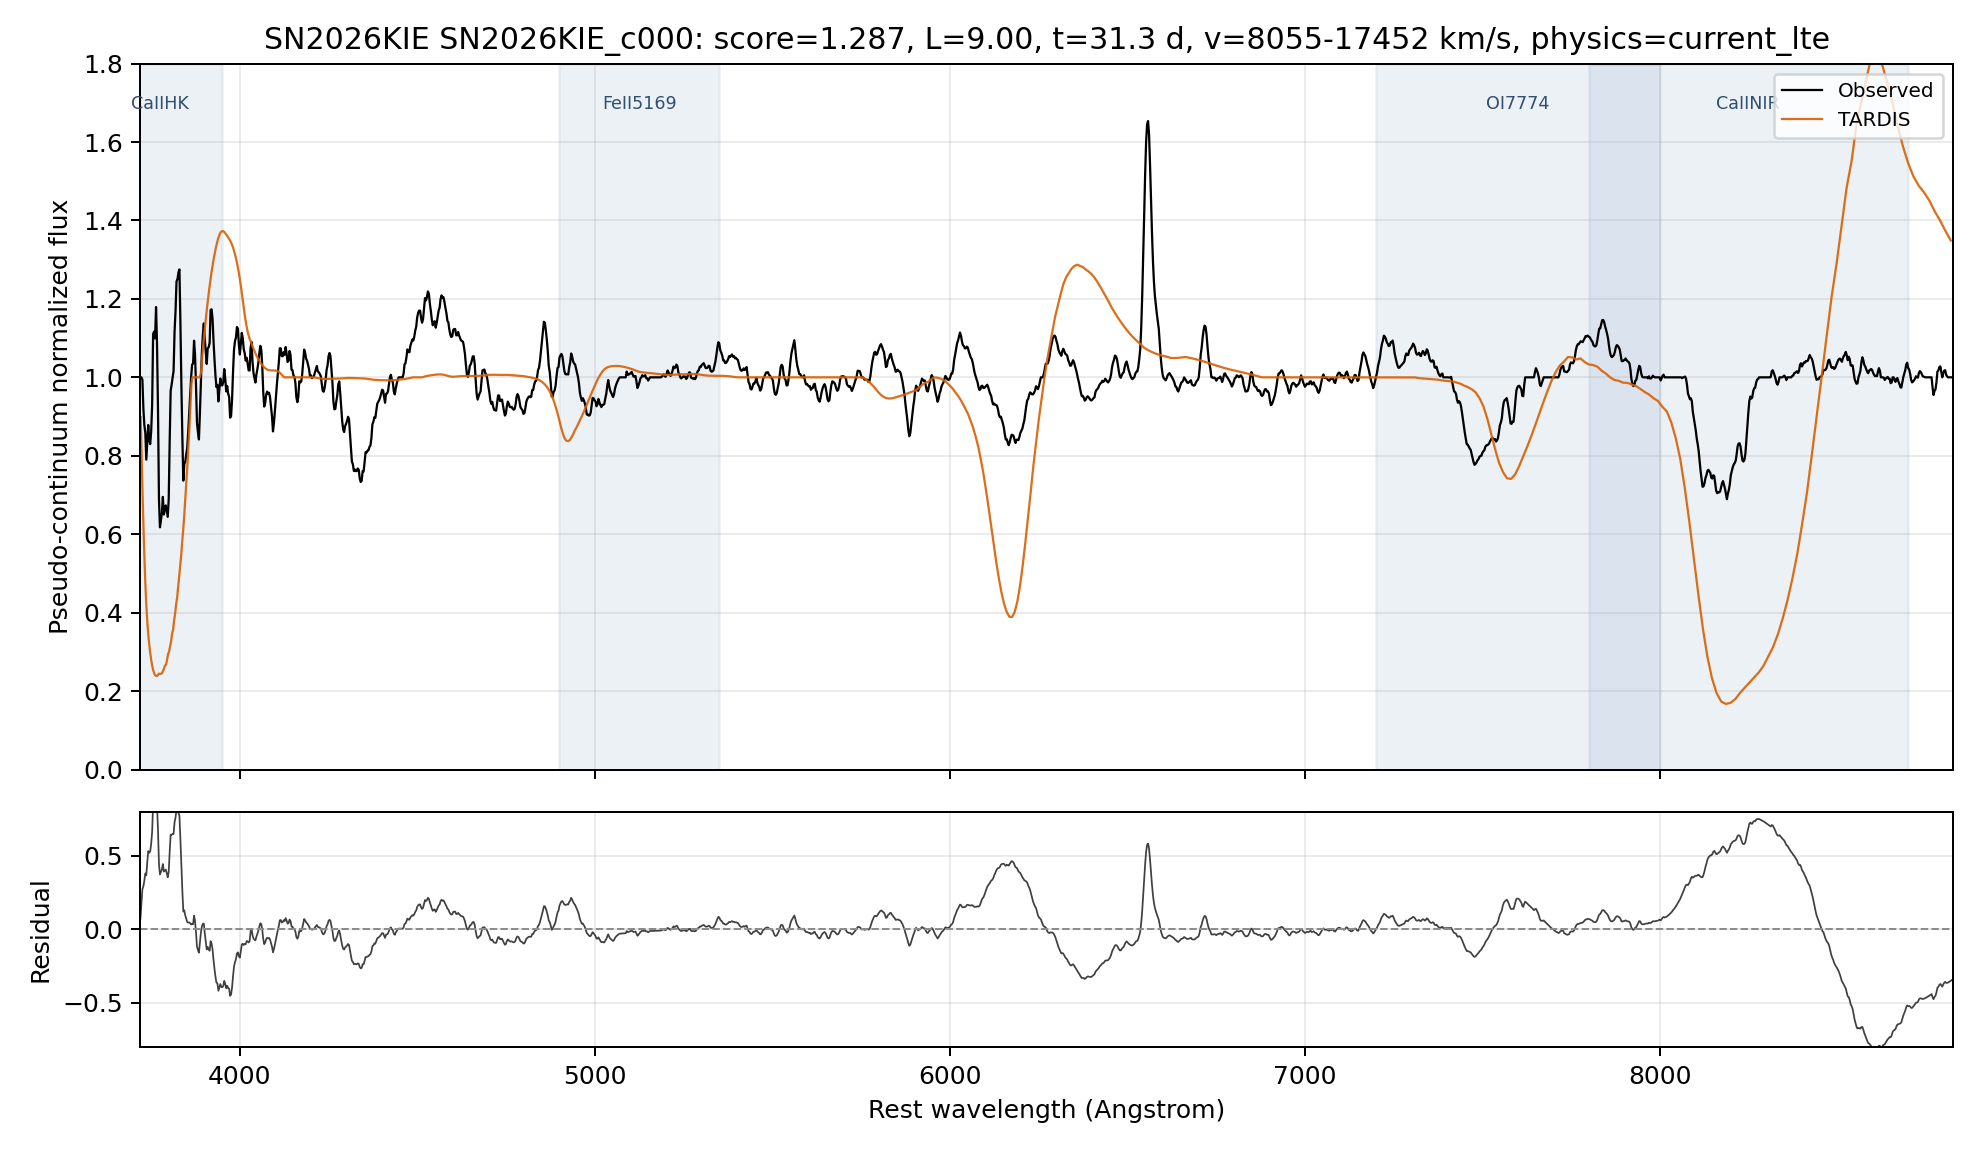
\includegraphics[width=0.95\linewidth]{images_zzzaurak/tardis_comparison_SN2026KIE.png}
\caption{Qualitative TARDIS comparison for SN2026KIE. The model partly reproduces the O I and Ca II regions but is not suitable for strong physical-parameter interpretation. From code by Ziheng Zhang.}
\label{fig:tardis-kie}
\end{figure}

Overall, TARDIS and the empirical line measurements play complementary roles. The empirical measurements provide the main quantitative results: velocities, pEW, FWHM, and the QC table. TARDIS checks whether the line identifications and velocity ranges can be produced by plausible one-dimensional ejecta models. The science conclusions should therefore rely primarily on the adopted line tables, while the TARDIS figures are best treated as qualitative supporting diagnostics.

\subsection{Limitations of This Section}
\begin{enumerate}[leftmargin=1.4em]
    \item This section starts from reduced one-dimensional spectra and does not redo the two-dimensional reduction, so the original reduction-error details are not fully available.
    \item Line velocities depend on the TNS redshift. SN2026LMP, which lacks a redshift, is not used quantitatively.
    \item The trough-minimum method is more direct than Gaussian fitting, but it still depends on the window, smoothing scale, and local-continuum definition. In blended broad-line regions, the systematic pEW uncertainty may be larger than the formal uncertainty listed in the tables.
    \item The TARDIS models fit only one representative spectrum per supernova, use simplified abundance presets, and do not perform multi-epoch joint fitting or true stratified abundance inversion.
    \item This section provides empirical diagnostics and qualitative radiative-transfer checks for sparse spectra; it is not a complete physical fit. The TARDIS results should be treated as supporting evidence rather than the main evidence chain.
\end{enumerate}

\section{Conclusion}

\printbibliography[title={References}]

\end{document}
